\documentclass[a4paper,11pt,minitoc,gray,chapterstyletwo,twoside,loabychapter,lotbychapter,lofbychapter]{NusThesis}    
%% class option:
%% loabychapter      : separate the list of algorithms by chapter
%% lotbychapter      : separate the list of tables     by chapter
%% lofbychapter      : separate the list of figures    by chapter
%% lolbychapter      : separate the list of codes      by chapter // use lstlisting environment
%% gray              : change colors to gray style
%% chapterstyletwo   : another type of chapter style
%% chapterstylethree : third type of chapter style
%% minitoc           : create a minitoc at each chapter

%% all the options for the book class can be added here

%% self defined commands and configurations and extra loaded packaged, which are not necessary 
%% to use this class
%%%%%%%%%%%%%%%%%%%%%%%%%%%%%%%%%%%%%%%%%%%%%%%%%%%%%%%%%%%%%%%%%%%%%%%%%%%%%%% 
% ams packages                                                                %
%%%%%%%%%%%%%%%%%%%%%%%%%%%%%%%%%%%%%%%%%%%%%%%%%%%%%%%%%%%%%%%%%%%%%%%%%%%%%%% 
                                                                                    
 \usepackage{amsmath,amsfonts,amssymb,amsthm,mathrsfs}

\usepackage{mathtools}
\usepackage{booktabs}
%%%%%%%%%%%%%%%%%%%%%%%%%%%%%%%%%%%%%%%%%%%%%%%%%%%%%%%%%%%%%%%%%%%%%%%%%%%%%%%
%                                    fonts                                    %
%%%%%%%%%%%%%%%%%%%%%%%%%%%%%%%%%%%%%%%%%%%%%%%%%%%%%%%%%%%%%%%%%%%%%%%%%%%%%%%
\usepackage[T1, OT1]{fontenc}
\DeclareTextSymbolDefault{\DH}{T1}
\DeclareTextSymbolDefault{\DJ}{T1}
    \usepackage{braket} 
%%%%%%%%%%%%%%%%%%%%%%%%%%%%%%%%%%%%%%%%%%%%%%%%%%%%%%%%%%%%%%%%%%%%%%%%%%%%%%%
%                                  refs                                       %
%%%%%%%%%%%%%%%%%%%%%%%%%%%%%%%%%%%%%%%%%%%%%%%%%%%%%%%%%%%%%%%%%%%%%%%%%%%%%%%
\usepackage{hyperref}
\usepackage[capitalize]{cleveref}
%%%%%%%%%%%%%%%%%%%%%%%%%%%%%%%%%%%%%%%%%%%%%%%%%%%%%%%%%%%%%%%%%%%%%%%%%%%%%%%
%                                 environments                                %
%%%%%%%%%%%%%%%%%%%%%%%%%%%%%%%%%%%%%%%%%%%%%%%%%%%%%%%%%%%%%%%%%%%%%%%%%%%%%%%
\usepackage{enumitem}
%%%%%%%%%%%%%%%%%%%%%%%%%%%%%%%%%%%%%%%%%%%%%%%%%%%%%%%%%%%%%%%%%%%%%%%%%%%%%%%
%                                    others                                   %
%%%%%%%%%%%%%%%%%%%%%%%%%%%%%%%%%%%%%%%%%%%%%%%%%%%%%%%%%%%%%%%%%%%%%%%%%%%%%%%
\usepackage{xspace}
\usepackage{tabstackengine}
%%% Local Variables:
%%% TeX-master: "thesis"
%%% End:
           % for used packages
%%%%%%%%%%%%%%%%%%%%%%%%%%%%%%%%%%%%%%%%%%%%%%%%%%%%%%%%%%%%%%%%%%%%%%%%%%%%%%% 
% self eivironment                                                            %
%%%%%%%%%%%%%%%%%%%%%%%%%%%%%%%%%%%%%%%%%%%%%%%%%%%%%%%%%%%%%%%%%%%%%%%%%%%%%%% 
\newtheorem{defi}{Definition}
\newtheorem{remark}{Remark}
\newtheorem{thm}{Theorem}
\newtheorem{corollary}[thm]{Corollary}
\newtheorem{question}{Question}
\newtheorem{proposition}[thm]{Proposition}
\newtheorem{lem}[thm]{Lemma}
\newtheorem{example}{Example}


%%%%%%%%%%%%%%%%%%%%%%%%%%%%%%%%%%%%%%%%%%%%%%%%%%%%%%%%%%%%%%%%%%%%%%%%%%%%%%% 
% symbols                                                                     %
%%%%%%%%%%%%%%%%%%%%%%%%%%%%%%%%%%%%%%%%%%%%%%%%%%%%%%%%%%%%%%%%%%%%%%%%%%%%%%% 
\usepackage{dsfont}
\newcommand{\I}{\mathds 1}
\newcommand{\real}{\mathbb{R}} 
\newcommand{\complex}{\mathbb{C}}
\newcommand{\natnumber }{\mathbb{N}}
\newcommand{\bbR}{\mathbb{R}}
\newcommand{\bbC}{\mathbb{C}}
\newcommand{\cP}{\mathcal{P}}
\newcommand{\cX}{\mathcal{X}}
\newcommand{\cH}{\mathcal{H}}
\newcommand{\iu}{\mathrm{i}\mkern1mu}

\newcommand{\ha}{\mathcal{H}_A} 
\newcommand{\hb}{\mathcal{H}_B} 
\newcommand{\hh}{\mathcal{H}}
\newcommand{\setS}{\mathcal{S}}%
\makeatletter
\newcommand{\notprop}{\propto\kern-1\@ptsize pt \diagup}
\makeatother

%%%%%%%%%%%%%%%%%%%%%%%%%%%%%%%%%%%%%%%%%%%%%%%%%%%%%%%%%%%%%%%%%%%%%%%%%%%%%%% 
% operators                                                                   %
%%%%%%%%%%%%%%%%%%%%%%%%%%%%%%%%%%%%%%%%%%%%%%%%%%%%%%%%%%%%%%%%%%%%%%%%%%%%%%% 
\newcommand{\rank}[1]{\mathrm{rank} (#1)} 
\newcommand{\range}[1]{\mathcal{R} (#1)}
\newcommand{\norm}[1]{\left\lVert#1\right\rVert} 
\newcommand{\kernel}[1]{\mathrm{Ker} (#1)}
\newcommand{\trace}[1]{\mathrm{Tr}(#1)}
\newcommand{\conj}[1]{\overline{#1}}
\newcommand{\adj}[1]{#1^{\mathsf{H}}}
\newcommand{\trans}[1]{#1^{\intercal}}
\newcommand{\Real}[1]{\mathrm{Re}(#1)}
\newcommand{\Ima}[1]{\mathrm{Im}(#1)}


% \DeclarePairedDelimiter\bra{\langle}{\rvert}
% \DeclarePairedDelimiterX\ket{\lvert}{\rangle}
% \DeclarePairedDelimiterX\braket[2]{\langle}{\rangle}{#1 \delimsize\vert#2}


%%%%%%%%%%%%%%%%%%%%%%%%%%%%%%%%%%%%%%%%%%%%%%%%%%%%%%%%%%%%%%%%%%%%%%%%%%%%%%% 
% abbreviated expression                                                      %
%%%%%%%%%%%%%%%%%%%%%%%%%%%%%%%%%%%%%%%%%%%%%%%%%%%%%%%%%%%%%%%%%%%%%%%%%%%%%%% 
\newcommand{\ei}[1][i]{\ket{#1}} % or e_i
\newcommand{\ej}{\ket{j}}
\newcommand{\xx}[1]{\adj{#1}#1}
\newcommand{\sijkl}[2]{S^1_{#1,#2}}
\newcommand{\sijklt}[2]{S^2_{#1,#2}}
\newcommand{\commutes}{\; \substack{\mathrm{commutes}\\
    \xrightarrow{\hspace*{6em}}\\ \mbox{}}\; }
\newcommand\lijkl[2]{\lambda^{1}_{#1 #2}}
\newcommand\lijklt[2]{\lambda^{2}_{#1 #2}}
\newcommand\Lijkl[1]{\Lambda^{1}_{#1 }}
\newcommand\Lijklt[1]{\Lambda^{2}_{#1}}

%% -------------------------------------------------- qed --------------------------------------------------
\renewcommand{\qedsymbol}{$\blacksquare$}

%% -------------------------------------------------- end --------------------------------------------------
%%%%%%%%%%%%%%%%%%%%%%%%%%%%%%%%%%%%%%%%%%%%%%%%%%%%%%%%%%%%%%%%%%%%%%%%%%%%%%% 
% abbreviations                                                                %
%%%%%%%%%%%%%%%%%%%%%%%%%%%%%%%%%%%%%%%%%%%%%%%%%%%%%%%%%%%%%%%%%%%%%%%%%%%%%%% 
\makeatletter
\DeclareRobustCommand\onedot{\futurelet\@let@token\@onedot}
\def\@onedot{\ifx\@let@token.\else.\null\fi\xspace}

\def\eg{\emph{e.g}\onedot} 
\def\Eg{\emph{E.g}\onedot}
\def\ie{\emph{i.e}\onedot} 
\def\Ie{\emph{I.e}\onedot}
\def\cf{\emph{c.f}\onedot} 
\def\Cf{\emph{C.f}\onedot}
\def\etc{\emph{etc}\onedot} 
\def\vs{\emph{vs}\onedot}
\def\wrt{w.r.t\onedot} 
\def\dof{d.o.f\onedot}
\def\etal{\emph{et al}\onedot}
\makeatother
\let\strokeL\L
\DeclareRobustCommand{\L}{\ifmmode\mathbf{L}\else\strokeL\fi}

%%%%%%%%%%%%%%%%%%%%%%%%%%%%%%%%%%%%%%%%%%%%%%%%%%%%%%%%%%%%%%%%%%%%%%%%%%%%%%% 
%          renewcommand                                                       % 
%%%%%%%%%%%%%%%%%%%%%%%%%%%%%%%%%%%%%%%%%%%%%%%%%%%%%%%%%%%%%%%%%%%%%%%%%%%%%%% 
\renewcommand{\intercal}{\mathsf{T}}
\renewcommand\tilde[1]{\stackrel{\sim}{\smash{{#1}}\rule{0pt}{1.1ex}}}


%





%%% Local Variables:
%%% mode: latex
%%% TeX-master: "thesis"
%%% End:
     % for delfdefined commands
%%  cinfiguration about the titles 
%%%%%%%%%%%%%%%%%%%%%%%%%%%%%%%%%%%%%%%%%%%%%%%%%%%%%%%%%%%%%%%%%%%%%%%%%%%%%%%  
%  Month year date                                                            %
%%%%%%%%%%%%%%%%%%%%%%%%%%%%%%%%%%%%%%%%%%%%%%%%%%%%%%%%%%%%%%%%%%%%%%%%%%%%%%%  

%%%%%%%%%%%%%%%%%%%%%%%%%%%%%%%%%%%%%%%%%%%%%%%%%%%%%%%%%%%%%%%%%%%%%%%%%%%%%%%
%                                   hypperref                                 %
%%%%%%%%%%%%%%%%%%%%%%%%%%%%%%%%%%%%%%%%%%%%%%%%%%%%%%%%%%%%%%%%%%%%%%%%%%%%%%%                                   
\hypersetup{unicode=true, % non-Latin characters in Acrobat’s bookmarks
  pdftoolbar=true, % show Acrobat’s toolbar?
  pdfmenubar=true, % show Acrobat’s menu?
  pdffitwindow=false, % window fit to page when opened
  pdfstartview={FitH}, % fits the width of the page to the window
  pdftitle={My title}, % title
  pdfauthor={Author}, % author
  pdfsubject={Subject}, % subject of the document
  pdfcreator={Creator}, % creator of the document
  pdfkeywords={keyword1, key2, key3}, % list of keywords
  pdfnewwindow=true, % links in new PDF window
  colorlinks=true, % false: boxed links; true: colored links
  linkcolor=blue, % color of internal links (change box color with linkbordercolor)
  citecolor=blue, % color of links to bibliography
  filecolor=blue, % color of file links
  urlcolor=blue, % color of external links
  pdfencoding=auto, psdextra 
}

%%% Local Variables:
%%% TeX-master: "thesis"
%%% End:
            % for specific configurations
%% users can replace the contents of the above files to these they need
%\usepackage{showframe}
%%%%%%%%%%%%%%%%%%%%%%%%%%%%%%%%%%%%%%%%%%%%%%%%%%%%%%%%%%%%%%%%%%%%%%%%%%%%%%% 
% input informations                                                          %
%%%%%%%%%%%%%%%%%%%%%%%%%%%%%%%%%%%%%%%%%%%%%%%%%%%%%%%%%%%%%%%%%%%%%%%%%%%%%%% 
\title{Quantum Entanglement}
\author{Qian Long}
\authordegree{B.Sc., Wuhan University}         % the degree has obtained 
\degree{Doctor of Philosophy}                  % degree this thesis for
\department{Department of Mathematics}         % current department 
\university{National University of Singapore}  % current university name
\declarationdate{\today}                       % declaration date
\supervisor{Associate Professor In Jen}     % Supervisor 
\examinerone{Professor A}          % three examiners, if not in your university,
\examinertwo{Professor B}          % may add the name of his university
\examinerthree{Professor C, University of Somecity}



% documents starts==============================================>
\begin{document}
\frontmatter              % change page number to roman number
\maketitle                % create title page 
\pagestyle{empty}
\AddDeclaration[signature2]% input tha fig name of your signature in the braket
\begin{acknowledgments}
I would like to express the deepest gratitude to my supervisors Prof. Chu Delin.

Besides my supervisors, I would like to express my sincere gratitude to Prof.
Chen Lin from Beihang University, P.R.China.


\begin{flushright}
  \textbf{\theauthor}\\
  \textbf{\the\year}
\end{flushright}

\end{acknowledgments}

%%% Local Variables:
%%% mode: latex
%%% TeX-master: "thesis"
%%% End:
   % input the contents of acknowledgement
\tableofcontents          % Table of contents.

%%%%%%%%%%%%%%%%%%%%%%%%%%%%%%%%%%%%%%%%%%%%%%%%%%%%%%%%%%%%%%%%%%%%%%%%%%%%%%% 
% summary                                                                     %
%%%%%%%%%%%%%%%%%%%%%%%%%%%%%%%%%%%%%%%%%%%%%%%%%%%%%%%%%%%%%%%%%%%%%%%%%%%%%%% 
\begin{summary}           % Summary of the thsis
  This dissertation contains two parts. Part I dedicates to develop
  risk analysis tool.
\end{summary}

%%% Local Variables:
%%% mode: latex
%%% TeX-master: "thesis"
%%% End:
           % input the contents of summary
\listoffigures            % create the list of figures and add to toc
\listoftables             % create the list of tables and add to toc
\listofsymbols            % create the list of symbols and add to toc. see symbols.tex for examples
\listofalgorithms         % create the list of algorithms and add to toc
\lstlistoflistings        % create the list of codes and add to toc
\listofpublications{Qian_sppt,Qian_CS,Qian_CS2} 

% create the list of your publication, 
% the contents if defined in contents file
%% main contents start========================================>
\mainmatter              % change page number to arabic number
\chapter*{Introduction}
\addstarredchapter{Introduction} % add the introduction to toc
%%% Local Variables:
%%% mode: latex
%%% TeX-master: "thesis"
%%% End:
     % introcution part
\pagestyle{circle}   % use to change the head and foot style
%% possible head style : basicstyle, gray, circle, circle2, circle3


% -------------------------------------------------- new theorem --------------------------------------------------



\chapter{SPPT states}
\section{Introduction}
Entanglement lies at the heart of quantum computation and information theory, which is the resource of most
applications in quantum information processing tasks.  Since 1935, when the necessarily nonlocal nature of quantum mechanics was
first highlighted by Einstein, Podolsky, and Rosen (EPR)~\cite{einstein1935can}, quantum entanglement has become a major
quantum phenomenon  which requires further understanding. One of the fundamental tasks about quantum entanglement is the
 separability problem, i.e.,  to check whether a given quantum state is separable.  Given a density
matrix $\rho$ in a quantum bipartite system $A:B$,   it is  said to be separable if it can be written as a convex combination
of product states~\cite{Werner1989},  i.e., 
\begin{align}
  \label{intro}
  \rho=\sum_i p_i\rho_i^A\otimes\rho_i^B,\;\sum_i p_i = 1,p_i\geqslant 0,
\end{align}
where $\rho_i^A$ and $\rho^B_i$ are density matrices  in subsystem A and  B respectively. A quantum state is said to be
 entangled if it does not possess a decomposition of the form as \cref{intro}. In this case, 
 the state cannot  be prepared by the  information of its two subsystems~\cite{Peres1996a}.


Despite  remarkable efforts over recent years, the operational necessary and sufficient condition for the
separability   remains unknown in general. It was found that the separable problem is NP-HARD even for
the bipartite system~\cite{gurvits2003classical}.

Although it is hard to solve this problem in general, there are plenty of  practical criteria which enable us to detect
entanglement for some subclasses.  One of the most famous criteria  is called positive
partial transpose (PPT)  or Peres-Horodecki criterion~\cite{Peres1996a}.  It tells  that if a state
$\rho$ is separable, then its partial transposed state $\rho^{\intercal_{A}} = (\intercal \otimes\I)\rho$ must remain
positive.
Using positive
maps, Horodecki {\sl et al.}~\cite{horodecki1996separability} showed that Peres-Horodecki criterion is also sufficient
for $2\otimes 2$ and $2\otimes 3$  systems. However, it fails in  higher dimensional spaces.
Woronowicz~\cite{Woronowikz1976} constructed a counterexample of a $2\otimes 4$ entangled PPT state. See more entangle
PPT states in Refs.~\cite{Choi1982,Strmer1963,Horodecki1997}.  Utilizing matrix analysis, Kraus {\sl et \
  al.}~\cite{Kraus2000} showed that any $M\otimes N (M\leqslant N)$  PPT state of rank $N$ is separable. Moreover, some generalized
results  are proposed in Refs.~\cite{Horodecki2000,Karnas2001,Fei2003}. Since any $M\otimes N$ state of rank less than
$N$ is distillable~\cite{horodecki2003rank}, it suffices to consider such state whose rank is greater than its local
ranks.


A subclass of PPT states, namely strong PPT (SPPT) states, were first considered by  {Chru\'sci\'nski} {\sl
  et al.}~\cite{Chruscinski2008}. These states have a ``strong PPT property''. Based on several examples, it was
conjectured that SPPT states are separable. Unfortunately, this conclusion fails for  $M\otimes N$ PPT states when
$NM\geqslant 9$. Actually, all $2\otimes 4$ SPPT states are separable~\cite{Ha2012}. But, there exists a $2\otimes 5$ SPPT
which is entangled~\cite{Ha2012}. The separability of SPPT states become more complex in high dimensional spaces. The
SPPT states encompass many previously known separable PPT states such as rank $N$ states of $2\otimes N$
system. Moreover, it is proved that SPPT states can be used to witness quantum discord (QD) in $2\otimes N$
systems~\cite{Bylicka2010}.  In addition, Bylicka {\sl et al.}~\cite{Bylicka2013} constructed  a special class of SPPT
states, which were called super strong SPPT (SSPPT) states.  In Ref.~\cite{Guo2012}, the
decomposition of SSPPT states was considered in both finite and infinite dimensional systems.


In a recent paper\cite{SPPT3partite}, the idea of SPPT states was generalized to the tripartite system
$A_{1}:A_{2}:A_{3}$. However, these states are essentially  bipartite SPPT  with respect to the bi-partition
$A_{1}A_{2}:A_{3}$. As a result, some good properties may be lost in the tripartite sense. For instance, 
the SPPT cannot guarantee PPT, which is one of the
most important features for SPPT states in the bipartite system.
Also, the super SPPT cannot  guarantee the separability in general.
Therefore, it would be especially interesting to find a more appropriate generalization to tripartite or even
multipartite systems.  The purpose of this paper is to provide an alternative definition of SPPT states in the multipartite
system. We begin with the simplest case when $\rho $ is in $2\otimes 2 \otimes N $,  and eventually, extend  to general many-body
system.


The remainder of this paper is organized as follows.  In Section~\ref{sec:preliminaries}, we present some preliminaries
about the separability problem of the SPPT states. In Section~\ref{sec:old-version-sppt}, we recall the definition of
tripartite SPPT states in Ref.~\cite{SPPT3partite}. We show that the defined SPPT and SSPPT cannot inherit some good
properties as those in the bipartite case.  In Section~\ref{sec:mySPPT}, we provide a new idea to define the SPPT and
SSPPT state in $2\otimes 2 \otimes N$ system.  We extend this concept to
$N_1\otimes N_2\otimes N_3$ case. Finally, we show  the idea  to the arbitrary multipartite system.
In Section~\ref{sec:suff-cond-sppt}, we  propose
some  sufficient conditions for separability of SPPT states. Some concluding remarks are given in \Cref{conclusion}.


\section{preliminaries}
\label{sec:preliminaries}
We start this section with a formal definition of separability.  Consider a $d$-particle state belonging to a Hilbert
space $\mathcal{H}$. Denote by $A_1$, $A_2$, $\cdots$, $A_d$ the subsystems respectively.  Each subsystem is a Hilbert
space $\mathcal{H}_i$ with dimension $N_i$. By the postulate for composition of system in quantum computation theory, we have
$\mathcal{H} = \otimes_{i=1}^d \mathcal{H}_i$ and $\dim(\mathcal{H})=\prod_{i=1}^{d}N_i$.

To make more concise, we use vector based indexes in this paper especially when the number of parties is large. Let
$\mathcal{I}$ be the set consisting of the  d-tuples
$ (i_1,i_2,\ldots,i_d),1\leqslant i_k\leqslant N_k$. For any given index $\alpha= (i_1,i_2,\ldots,i_d)\in \mathcal{I}$, 
$x_{\alpha}$ represents $x_{i_1,i_2,\ldots,i_{d}}$. Furthermore, we  assign an order for those indexes. Let
\[
  \pi(\alpha)= \prod_{k=1}^{d-1}(\prod_{l=k+1}^{d}N_l)(\alpha_k-1)+\alpha_d.
\]
 For $\alpha,\beta\in \mathcal{I}$, $\alpha< \beta (\alpha\leqslant \beta)$ denotes $\pi(\alpha)<\pi(\beta)(\pi(\alpha)\linebreak\leqslant \pi(\beta))$. For example, in the bipartite case, $(i,j)<(k,l)$ equals $(i-1)N_2+j<(k-1)N_2+l$.  Moreover, $\ket{\alpha} $ represents the product vector $\ket{i_1,i_2,\ldots,i_d}$.

Hence a density matrix acting on the space $\mathcal{H}$ can be represented as
\begin{equation}
  \label{eq:37}
  \rho = \sum_{\alpha,\beta\leqslant \alpha_0}  \rho_{\alpha,\beta}| \alpha\rangle \langle \beta|, 
\end{equation}
where $\alpha,\beta\in\mathcal{I}$ and $\alpha_0 = (N_1,N_2,\ldots,N_d)$.

Now we recall the definition of separability of a quantum state. A density matrix $\rho$ acting on  $\mathcal{H}$ is said to be
separable if it can be written as
\begin{equation}
  \label{eq:12}
  \rho = \sum_{i=1}^{L} \lambda_i\ket{x_i}\bra{x_i},
\end{equation}
where $\sum_{i}^{L}\lambda_i = 1,\lambda_i\geqslant 0$ and each $\ket{x_{i}}$ is a pure product vector in the space
$\mathcal{H}$.

Peres-Horodecki criterion plays a crucial role in the separability problem, which is based on the partial transpose.
Therefore it would be necessary to introduce the notations of partial transposes before going further.  Denote by $\intercal$ the usual transpose operator.  Then the composite
operators $(\I\otimes \intercal)$ and $(\intercal\otimes \I)$ are called the partial transpose operators in the
bipartite system. Furthermore,
the partial transposed density matrices are denoted by $ \rho^{\intercal_2}=(\I\otimes \intercal)\rho$ and
$\rho^{\intercal_1}=(\intercal\otimes \I)\rho $ respectively.  For general multipartite system $A_1:A_2\cdots:A_d$, denote by
$\intercal_i$ ( $i=1,2,\ldots,d$) the partial transpose with respect to $i$-th subsystem respectively. The corresponding
partial transposed state is denoted by $\rho^{\intercal_i}$. Generally, for any  given  index set $I = \{i_1,i_2,\ldots,i_k\}$,
let $\intercal_I$ denote the partial transpose with respect to the subsystems in $I$, that is
\[ \intercal_{I}= \circ_{k\in I}\intercal_k.\] 

PPT  criterion tells  that if $\rho$ is separable, then
\begin{equation}
  \label{multiSPPTv0.6:eq:1}
  \intercal_{\!I} \cdot \rho\geqslant 0,\,\forall I\subset \{1,2,\ldots,d\}.
\end{equation}

Now we recall the definition of SPPT in the bipartite system.



Consider a density matrix $\rho$ in $N_1\otimes N_2$ system which has a block Cholesky decomposition $\rho = \adj X X$:
\begin{equation}
  \label{eq:40}
  \begin{split}
    X&=
    \begin{pmatrix}
      S_{11}X_1 &\cdots&S_{1N_1}X_1\\
      \vdots&\ddots& \vdots\\
      S_{N_1 1}X_{N_1}&\cdots&S_{N_1N_1}X_{N_1}\\
    \end{pmatrix}\\
    & =
    \begin{pmatrix}
      X_1 &\cdots&S_{1N_1}X_1\\
      \vdots&\ddots& \vdots\\
      0&\cdots&X_{N_1}\\
    \end{pmatrix},
  \end{split}
\end{equation}
where $S_{ij}$ and $X_i$ are both $N_2\times N_2$ matrices with
\begin{equation*}
  S_{ij} =
  \begin{cases}
    \I_{N_2}, & \text {if } i=j;\\
    0, & \text{if }i > j.
  \end{cases}
\end{equation*}
In this paper,    $\I_n$ denotes the identity operator acting on the space $\complex^n$. It is also written   
as $\I$ when there is no doubt about the dimension.
\begin{defi}
  Let $\rho$ be a density matrix in $N_1\otimes N_2$ system. And $\rho = \adj X X$, where $X$ has the form as
  \cref{eq:40}. Then $\rho$ is said to be SPPT if
  \begin{equation}
    \label{eq:41}
    \rho^{\intercal_1} = \adj Y Y,
  \end{equation}
  with
  \begin{equation*}
    Y =
    \begin{pmatrix}
      S^\dagger_{11}X_1&\cdots &S^\dagger_{1N_1}X_1\\
      \vdots&\ddots&\vdots\\
      S^\dagger_{N_11}X_1&\cdots&S^\dagger_{N_1N_1}X_1\\
    \end{pmatrix},
  \end{equation*}
  or equivalently,
  \begin{equation}
    \label{eq:42}
    \sum_{k=1} ^{N_1} \adj X_k [\adj S_{kj},S_{ki}]X_k = 0,\;1\leqslant i \leqslant j\leqslant N_1.
  \end{equation}
\end{defi}

Here the commutator  $[A,B]$ is defined by $[A,B]= AB-BA$.

In particular, \cref{eq:42} is naturally satisfied if
\begin{equation}
  \label{eq:43}
  [\adj S_{kj},S_{ki}]=0,1\leqslant i, j\leqslant N_1.
\end{equation}
These states are named   super SPPT (SSPPT) states~\cite{Chruscinski2008}, which are proved to be  separable~\cite{Bylicka2013}.
        




\section{Previous definition of tripartite SPPT states}%
~\label{sec:old-version-sppt}
In this section, firstly we will  introduce the definition of tripartite SPPT states in Ref.~\cite{SPPT3partite}.
After that, we will show that these SPPT states will not preserve some good properties as that in the bipartite system. For
example, the SPPT state may not be PPT.\@ Besides, pure or super SPPT states may not be separable.

Suppose  $\rho$ is a density matrix in the tripartite system  $A_1:A_2:A_3$, which has a
decomposition $\rho = \adj X X$. Under the bi-partition $A_1:A_2A_3$, $X$ can be written as an $N_1\times N_1$ block matrix:
\begin{equation}
  \label{eq:44}
  X =
  \begin{pmatrix}
    Z_{11}&\cdots&Z_{1N_1}\\
    \vdots &\ddots&\vdots\\
    Z_{N_11}&\cdots&Z_{N_1N_1}\\
  \end{pmatrix},\;Z_{ij}\in\complex^{N_2N_3\times N_2N_3}.
\end{equation}
Again, each $Z_{ij}$ can be  written as an $N_2\times N_2$ block matrix:
\begin{equation}
  \label{eq:45}
  Z_{ij} 
  =
  \begin{pmatrix}
    S_{ij11}X_{i1}&\cdots&S_{ij1N_2}X_{i1}\\
   \vdots &\ddots &\vdots \\
    S_{ijN_21}X_{iN_2}&\cdots&S_{ijN_2N_2}X_{iN_2}
  \end{pmatrix},
\end{equation}
where
\begin{equation}
  \label{eq:46}
  S_{ijkl} =
  \begin{cases}
    \I_{N_3}, & (i,k) = (j,l);\\
    0,& (i,k) > (j,l).
  \end{cases}
\end{equation}
Let $\alpha = (i,k),\beta = (j,l)$, then
\begin{equation}
   \label{eq:1}
 \rho = \adj  X X,
\end{equation}
in which  the $(\alpha,\beta)$-th entry of $X$ is $S_{\alpha,\beta}X_\alpha$. For simplicity,  let $(\alpha,\beta)$-th entry denote  the element in $\pi(\alpha)$-th row and $\pi(\beta)$-th column of a block matrix.

Recall the definition of SPPT state in Ref.~\cite{SPPT3partite}:
\begin{defi}
  Let $\rho=\adj XX$ be a density matrix in the tripartite system $A_1:A_2:A_3$ with $X$ being of  the form as \cref{eq:1}. Then
  $\rho$ is said to be  SPPT if
  \begin{equation}
    \label{eq:4}
    \rho^{\intercal_{12}} = \adj{Y} Y,
  \end{equation}
  where the $(\alpha,\beta )$-th entry of $Y$ is $S^\dagger_{\alpha,\beta}X_\alpha$.
\end{defi}

Note that in the above definition, the condition~\eqref{eq:4} is equivalent to
\begin{equation}
  \label{eq:5}
  \sum_{\gamma_0\leqslant \alpha\leqslant \gamma_1} \adj{X_{\alpha}}\left[S_{\alpha,\beta},\adj{S_{\alpha,\beta'}}\right] X_{\alpha}=0,
\end{equation}
where  $\gamma_0 = (1,1)$, $\gamma_1  = (N_1,N_2)$,  and $\gamma_0 \leqslant\beta\leqslant\beta'\leqslant \gamma_1$.

Similarly, super SPPT (SSPPT) are also defined for tripartite system in Ref.~\cite{SPPT3partite}.
\begin{defi}
  Let $\rho$ be an SPPT state with a decomposition as in \cref{eq:1}, then $\rho$ is said to be SSPPT if
  \begin{equation}
    \label{ssppt3}
    [S_{\alpha,\beta},\adj S_{\alpha,\beta'}] = 0, \; \gamma_0\leqslant\alpha\leqslant \beta \leqslant \beta' \leqslant \gamma_1.
  \end{equation}
\end{defi}

Note that $\alpha$ refers to the $n(\alpha)$-th row and $\beta$ refers to the $n(\beta)$-th column. Therefore, if we
reorder the 2-tuple $\alpha,\beta$ by $n(\alpha)$ and $n(\beta)$ respectively, then the definition of
SPPT will be identical to that in the bipartite system $A_1A_2:A_3$. Consequently, the same  properties  may not be kept in
tripartite system.  

 PPT, for instance,  is one of the most important features for SPPT states. However, the tripartite SPPT states
 defined this way may lose it. Here we construct an example to show this defect.

Let
\begin{equation*}
 \rho = \adj v v,\; v = (1,0,0,0,0,0,1,0),
\end{equation*}
which is an entangled state in  $2\otimes  2\otimes 2$ system.

In order to prove that  it is  an SPPT state, let 
\begin{equation}
  \label{multiSPPTv0.6:eq:14}
  X_{11} =
  \begin{pmatrix}
    1&0\\
    0&0
  \end{pmatrix},
  X =
  \begin{pmatrix}
    X_{11} & 0 & 0 & X_{11}\\
    0&0&0&0\\
    0&0&0&0\\
    0&0&0&0
  \end{pmatrix}.
\end{equation}
Then $\rho$ can be written as
\begin{equation}
  \label{multiSPPTv0.6:eq:15}
  \rho = \adj X X.
\end{equation}
Put
\begin{equation}
  \label{multiSPPTv0.6:eq:16}
  S_{\alpha,\beta} =
  \begin{cases}
    \I , &\text{if } \alpha=\beta = (1,1),\\
    0,&\text{otherwise}.
  \end{cases}
\end{equation}
By checking the conditions~\eqref{ssppt3}, $\rho$ is SSPPT.\@ However, it is not PPT since any pure PPT state is separable. Moreover, this example 
implies that  super and pure SPPT states may not be separable.




In  Theorem 1 of Ref.~\cite{SPPT3partite}, the authors pointed out that any SSPPT state is bi-separable.
It should be noted  that the  tripartite SSPPT states are bi-separable only with respect
to  the  bi-partition $A_1A_2:A_3$. Consider the example $\rho = \adj v
v$ again. It is  SSPPT by definition but  not separable under either the  bi-partition  $A_1:A_2A_3$ or $A_1A_3:A_2$.

In the next section, we will define our SPPT
and SSPPT states in another way. It turns out  that  many desired properties will be preserved. 

\section{SPPT states in  multipartite case}%
\label{sec:mySPPT}%
In this section, we provide an alternative way to define the tripartite SPPT states.  
The main idea is to require the states to satisfy   SPPT conditions  under a series of bi-partitions. As a result, these
states will remain positive under any partial transpose. 
Moreover, some other properties are also preserved compared with the previous definition in \cite{SPPT3partite}.

We begin with the simplest case $2\otimes 2
\otimes N$, then we extend the idea to general $N_1\otimes N_2\otimes N_3$ tripartite system. Lastly, we give the
definition of SPPT in the arbitrary multipartite system. Correspondingly, the SSPPT states are also introduced, which turn
out to be separable. In addition, we give some examples of SPPT states, which may be helpful to  shed new lights on
understanding the structure of PPT states in multipartite system.


\subsection{SPPT states in \texorpdfstring{$2\otimes 2 \otimes N$}{TEXT} system}
We begin with the simplest case when $\rho$ is a density matrix in $2\otimes 2 \otimes N$ system.
This can serve as  an example to show the intuition of generalization for many body system.

Let $\rho$ be a density matrix with $\rho = \adj{X}X$. In order to keep PPT, we require $\rho$ to be SPPT under either
the  bi-partition $A_1:A_2A_3$ or $A_1A_2:A_3$. For $A_1:A_2A_3$,  $X$ should be an upper triangular block matrix as
\begin{equation}
  \label{eq:15}
  X =
  \begin{pmatrix}
    X_1 & SX_1\\
    0 & X_2
  \end{pmatrix}.
\end{equation}
Under bi-partition $A_1:A_2A_3$, $X$ should have the following  upper triangular block representation:
\begin{equation*}
  \begin{split}
    X&=
    \begin{pmatrix}
      X_{11} & R_{1112}X_{11} & R_ {1121}X_{11} & R_{1122}X_{11} \\
 0 &X_{12} & R_ {1221}X_{12} & R_{1222}X_{12} \\
  0 & 0 & X_{11} & R_{2122}X_{21} \\
 0 & 0 &0 & X_{22}
\end{pmatrix}\\
&=
    \begin{pmatrix}
  R_{1111}X_{11} & R_{1112}X_{11} & R_ {1121}X_{11} & R_{1122}X_{11} \\
  R_{1211}X_{12} & R_{1212}X_{12} & R_ {1221}X_{12} & R_{1222}X_{12} \\
  R_{2111}X_{21} & R_{2112}X_{21} & R_ {2121}X_{11} & R_{2122}X_{21} \\
  R_{2211}X_{22} & R_{2212}X_{22} & R_ {2221}X_{22} & R_{2222}X_{22}
\end{pmatrix},
\end{split}
\end{equation*}
where
\begin{equation*}
  \label{multiSPPTfinal2:eq:2}
  R_{ijkl} =
  \begin{cases}
    \I_N, &\text{ if }(i,j) = (k,l),\\
    0,& \text{ if }(i,j)>(k,l).
  \end{cases}
\end{equation*}
In order to have the above form , we require
\begin{align*}
  X_1 =
  \begin{pmatrix}
    X_{11} & T_1 X_{11}\\
    0 & X_{12}
  \end{pmatrix}, X_2 =
        \begin{pmatrix}
          X_{21} & T_{2} X_{21}\\
          0 & X_{22}
        \end{pmatrix}.
\end{align*}
And  $S$ should be a block diagonal matrix, i.e.,
\begin{equation*}
  S=
  \begin{pmatrix}
    S_1 & 0\\
    0& S_2
  \end{pmatrix}.
\end{equation*}
Hence, $X$ can  be written as a $4\times 4$ upper  triangular block matrix with each block being of size $N\times N$:
\begin{equation}
  \label{eq:16}
  \begin{split}
  X & =
  \begin{pmatrix}
    X_{11} & T_1 X_{11} & S_1X_{11} & S_1T_1 X_{11}\\
    0 & X_{12} & 0 & S_2X_{12}\\
    0 & 0& X_{21} & T_2 X_{21}\\
    0 & 0 & 0& X_{22}
  \end{pmatrix}.
  \end{split}
\end{equation}
Let
\begin{equation}
  \label{multiSPPTfinal2:eq:1}
   Y_1 =
  \begin{pmatrix}
    X_1 &\adj SX_1\\
    0 & X_2
  \end{pmatrix},
\end{equation}
and 
\begin{equation*}
  Y_2 =
  \begin{pmatrix}
    X_{11} & \adj T_1 X_{11} & \adj S_1X_{11} & \adj{(S_1T_1)} X_{11}\\
    0 & X_{12} & 0 & \adj S_2X_{12}\\
    0 & 0& X_{21} & \adj T_2 X_{21}\\
    0 & 0 & 0& X_{22}
  \end{pmatrix}.
\end{equation*}

 
Here we give the definition of  SPPT states in the $2\otimes 2\otimes N$ system formally.
\begin{defi}
  Let $\rho = \adj X X$ be a density matrix in  $2\otimes 2\linebreak\otimes N $ system where $X$ has the  form as in \cref{eq:16}. Then
  $\rho$ is said to be SPPT if 
  \begin{equation}
    \label{eq:17}
    \rho^{\intercal_1} = \adj{Y_1}\,Y_1 ,
  \end{equation}
  and
  \begin{equation}
    \label{eq:18}
    \rho^{\intercal_{12}} = \adj{Y_2}\,Y_2.
  \end{equation}
\end{defi}
Alternatively, the above two conditions in the definition of SPPT can be reformulated as
\begin{equation}
\label{eq19p}
\begin{split}
\adj X_1[S,\adj S]X_1 &= 0,\\
\sum_{i,k=1}^2 X^\dagger_{ik}[ R_{ijkl},R^\dagger_{ij'kl'}]X_{ik} &= 0.
\end{split}
\end{equation}
For this simple case, \cref{eq19p} can be written  explicitly as
\begin{equation}
  \label{eq:19}
  \left\lbrace
    \begin{aligned}
     & \adj X_{11} [T_1,\adj T_1] X_{11} &= 0,\\
      &\adj X_{11} [ S_1,\adj S_1] X_{11} & =0,\\
      &\adj X_{11}[T_1,\adj S_1] X_{11} & = 0,\\
       &\adj X_{11} [S_1,\adj S_1 ] T_1 X_{11}& = 0,\\
      &\adj X_{11} [ S_1,\adj T_1\adj S_1] X_{11} &  = 0,\\
      &\adj X_{11} [ T_1,\adj T_1\adj S_1] X_{11} & = 0,\\
            &\adj X_{11} \adj T_1[ S_1,\adj S_1]T_1 X_{11}+\adj{X}_{12}[S_2,\adj S_2]X_{12} & = 0,\\
      &\adj X_{11} [ S_1T_1,\adj{(S_1T_1)}] X_{11} \\
      &\quad+ \adj X_{12}[  S_2,\adj S_2]X_{12} + \adj X_{21} [ T_2,\adj T_2] X_{21}&=0.\\
    \end{aligned}
  \right.
\end{equation}

Note that conditions~\eqref{eq:17} and~\eqref{eq:18} guarantee a ``strong PPT property''. This is one of the most different aspects compared with definition in previous section. 
Consider \cref{eq19p}, if all the  commutators vanishes, the SPPT conditions will be satisfied automatically. This class
of SPPT states are thus said to be super SPPT (SSPPT).
\begin{defi}
  Suppose  $\rho=\adj X X$ is an SPPT state where $X$ has form as in \cref{eq:16}. Then $\rho$ is called a SSPPT state if
  \begin{equation}
  \label{20pp}
  \begin{split}  
  	[S,\adj S] &= 0,\\
  	[R_{ijkl},R^\dagger_{ij'kl'}] &=0.
  	 \end{split}
  \end{equation}  
\end{defi}
In detail, \cref{20pp} can be written  as 
\begin{equation}
\label{eq:20p}
\left\lbrace
\begin{array}{rl}%
[S_i,\adj S_i] & = 0,i=1,2,\\
{[}T_i,\adj T_i] &= 0,i=1,2,\\
{[}S_1,\adj T_1] & = 0.\\
\end{array}
\right.
\end{equation}
 In the following theorem, we show that SSPPT can guarantee the separability.
\begin{thm}
  All SSPPT states in the tripartite system $2\otimes 2\otimes N$ are separable.
\end{thm}
\begin{proof}
According to \cref{eq:20p},   $ T_1,T_2,S_1,S_2$ are normal and $T_1$ commutes with $S_1$. Therefore, we have the
following   diagonalizations:
  \begin{equation}
    \label{eq:21p}
    \begin{split}
      S_1   & = U   \Sigma_{1}  \adj U,  T_1  = U   \Sigma_{2}  \adj U,\\
      S_2  & = V_1 \Lambda_{1} \adj V_1
      ,  T_2  = V_2 \Lambda_2 \adj V_2,\\
    \end{split}
  \end{equation}
  where $\Sigma_i,\Lambda_i$ are the diagonal matrices and $U$, $V_1$ and $V_2$ are
  all unitary matrices.  Then
  
  \begin{equation}
    \label{eq:22p}
    \begin{split}
      X &=
      \begin{pmatrix}
        U \adj U X_{11} &  U \Sigma_2 \adj U X_{11} & U \Sigma_1 \adj U  X_{11} & U\Sigma_1\Sigma_2 \adj U X_{11} \\
        0 &  V_1 \adj V_1 X_{12} & 0 & V_1 \Lambda_1 \adj V_1 X_{12}\\
        0 & 0 & V_2 \adj V_2 X_{21} &  V_2 \Lambda_2\adj V_2X_{21}\\
        0 & 0 & 0 & X_{22}\\
      \end{pmatrix}                    \\
      & =
      \begin{pmatrix}
        U & 0 & 0 &0 \\
        0 & V_2 & 0 &0 \\
        0 & 0 & V_1 & 0 \\
        0 & 0 & 0 & \I_N\\
      \end{pmatrix}
      \begin{pmatrix}
        \tilde X_{11} &   \Sigma_2\tilde X_{11} & \Sigma_1 \tilde X_{11} & \Sigma_1\Sigma_{2} \tilde X_{11} \\
        0 &  \tilde X_{12} & 0 &  \Lambda_1 \tilde X_{12}\\
        0 & 0 &  \tilde X_{21} &   \Lambda_2\tilde X_{21}\\
        0 & 0 & 0 & X_{22}\\
      \end{pmatrix}\\
      & = G \tilde X,
    \end{split}
  \end{equation}
 
  where
  \begin{equation}
    \label{eq:23p}
    \tilde X_{11} =  \adj U X_{11}, \tilde X_{12} =  \adj V_1 X_{12}, \tilde X_{21} =  \adj V_2 X_{21}.   
  \end{equation}
  
  Let
  \begin{equation*}
    \begin{array}{rclcccccrl}
      C_1 & = &\left(\right. &\tilde X_{11} &   \Sigma_2\tilde X_{11} & \Sigma_1 \tilde X_{11} & \Sigma_1\Sigma_{2} \tilde X_{11}&\left.\right)&, \\
      C_2 & = &\left(\right. &  0 &  \tilde X_{12} & 0 &  \Lambda_1 \tilde X_{12}&\left.\right)&,\\
      C_3 & = & \left(\right. &  0 & 0 &  \tilde X_{21} &   \Lambda_2\tilde X_{21}&\left.\right)&,\\
      C_4 & = & \left( \right.& 0 & 0 & 0 & X_{22}&\left.\right)&.\\
    \end{array}
  \end{equation*}
 Note that $\rho = \adj X X$ and $G$ is a unitary matrix,  then  we obtain,
  \begin{equation*}
    \rho = \sum_{i=1}^4\adj C_i C_i.
  \end{equation*}
  On the other hand,
  \begin{equation*}
    \begin{split}
      C_1 &= (\I,\Sigma_1)\otimes (\I,\Sigma_2) \otimes \tilde X_{11},\\
      C_2 & = (\I,\Lambda_1)\otimes (\,0\;,\I\,) \otimes \tilde X_{12},\\
      C_3 & = (\,0\;,\I\,)\otimes (\I,\Lambda_2) \otimes \tilde X_{21},\\
      C_4 &= (\,0\;,\I\,)\otimes (\,0\;,\I\,) \otimes \tilde X_{22}.
    \end{split}
  \end{equation*}
  It follows that each $\adj C_i C_i$ is separable, which implies the separability of $\rho$.
\end{proof}
  Note that this proof can also be regarded as a method to
  find the separability  decomposition of   $2\otimes 2\otimes N$ SSPPT states.

  Here we give an example of SPPT states in our definition.
  \begin{example}
     It was proved that if a PPT state  $\rho$ supported on $2\otimes 2\otimes N (N\geqslant 2)$ 
 has  rank $N $, then it  is separable and has the canonical form~\cite{Karnas2001}
 \begin{equation}
   \label{multiSPPTv0.6:eq:2}
   \rho = 
   \begin{pmatrix}
     \I_{N} \\ \adj B \\\adj C \\\adj B \adj C
   \end{pmatrix}
   \begin{pmatrix}
     \I_{N} & B & C & CB
   \end{pmatrix},
\end{equation}
where $B,C$ are normal commuting operators in the third subsystem.
  \end{example}

It is easy to check that
this canonical form is SPPT by definition. Forward, it is also an  SSPPT state.

\subsection{SPPT states in \texorpdfstring{$N_1\otimes N_2\otimes N_3$}{TEXT} tripartite system}
In this subsection we will extend the SPPT states to  general tripartite system $N_1\otimes N_2\otimes N_3$. The basic
idea is to  require $\rho$ to be SPPT under the bi-partition $A_1:A_2A_3$ and $A_1A_2:A_3$ simultaneously.

Let $\rho$ be the density matrix with a   decomposition $ \rho= \adj X X$ in the tripartite system $N_1\otimes N_2\otimes
N_3$.

Under the bipartite partition $A_1:A_2A_3$, $X$ can be written as an $N_1\times N_1$ block matrix:
\begin{equation}
  \begin{split}
  X
  = 
  \begin{pmatrix}
    X_1 & S_{12}X_1&\cdots &S_{1N_1}X_1\\
    0 & X_2&\cdots  & S_{2N_1}X_2\\
    \vdots &\vdots &\ddots &\vdots\\
    0 & 0  &\cdots& X_{N_1}\\
  \end{pmatrix}.
  \end{split}
\end{equation}

For consistent, let
\begin{equation}
  \label{multiSPPTv0.6:eq:3}
  S_{ij} =
  \begin{cases}
    0, &  \text{if } i>j,\\
    \I_{N_2N_3},& \text{if } i=j.
  \end{cases}
\end{equation}

Similarly, $X_i$ can
be written as an $N_2\times N_2$ block matrix:
\begin{equation*}
  \begin{split}
    X_i &=
    \begin{pmatrix}
      X_{i1} & \sijklt{i}{12}X_{i1} & \cdots &\sijklt{i}{1N_2}X_{i1}\\
      0 & X_{i2} & \cdots & \sijklt{i}{2N_2}X_{i2}\\
      \vdots & \vdots & \ddots & \vdots \\
      0 & 0 & \cdots & X_{iN_2}
    \end{pmatrix}   
  \end{split}
\end{equation*}
Here the superscript $2$ in the matrices $\sijklt{i}{kl}$ indicates the subsystem $A_2$ and let
\begin{equation*}
  \sijklt{i}{kl} =
  \begin{cases}
    \I_{N_3},& \text{if }  k=l;\\
    0, & \text{if } k>l.
  \end{cases}
\end{equation*}

In order to be compatible with the SPPT structure in the bipartite system $A_1A_2:A_3$, we require  $S_{ij}$ to be a block
diagonal matrix,
\begin{equation}
  \label{eq:7}
    S_{ij}  =
    \begin{pmatrix}
      \sijkl{ij}{1}& 0 & \cdots &0\\
      0 & \sijkl{ij}{2}&\cdots & 0\\
      \vdots & \vdots & \ddots & \vdots \\
      0& 0& \cdots & \sijkl{ij}{N_2}\\
          \end{pmatrix}.
        \end{equation}
 Hence
 \begin{equation}
   \begin{split}
     \rho &= \adj X X,
    \end{split}
   \label{sppt}
 \end{equation}
 where the $(N_2(i-1)+j,N_2(k-1)+l)$-th entry of $X$ is $$\sijkl{ij}{k} \sijklt{i}{kl} X_{ik}.$$
 Let \begin{align}
 	Y_1	=  \begin{pmatrix}
 	X_1 & \adj S_{12}X_1&\cdots &\adj S_{1N_1}X_1\\
 	0 & X_2&\cdots  & \adj S_{2N_1}X_2\\
 	\vdots &\vdots &\ddots &\vdots\\
 	0 & 0  &\cdots& X_{N_1}\\
 	\end{pmatrix},
 \end{align}
 and $Y_2$ be an $N_1N_2\times N_1N_2$ block matrix whose $(N_2(i-1)+j,N_2(k-1)+l)$-entry is
 \begin{align}
 \adj{(\sijklt{i}{kl})} \;\adj{(\sijkl{ij}{k} ) } \;X_{ik}.
 \end{align}
 
Now we are ready to define the SPPT state in general tripartite system with the matrices introduced above.
\begin{defi}
  Let $\rho$ be the density matrix in the tripartite system  $A_1:A_2:A_3$, and has a    decomposition 
  of the form as in \cref{sppt}. Then  $\rho$ is said to be  SPPT if 
  \begin{align}
  	\rho^{\intercal_1} = \adj{Y_1}\,Y_1,
  \end{align}
  and \begin{align}
  	\rho^{\intercal_{1,2}} = \adj{Y_2}\,Y_2.
  \end{align}
\end{defi}

Note that the above conditions required for SPPT are equivalent to the following   matrix equations:
\begin{equation}
  \label{eq:24}
  \begin{split}
    \sum_{i=1}^{N_1} \adj X_i [S_{ip},\adj S_{iq}]X_i & = 0,\\
    \sum_{i=1}^{N_1}\sum_{k=1}^{N_2} \adj X_{ik}   [ \sijkl{ij}{k}\sijklt{i}{kl},  \adj{(\sijkl{ij'}{k}\sijklt{i}{kl'}) }]
    X_{ik} &= 0 .
  \end{split}
\end{equation}

It is clear from the definition that  SPPT states defined here are indeed PPT, i.e.\ positive under any partial
transpose. Moreover,  \cref{eq:24} will be satisfied if all the commutators vanishes. Similarly to the previous
subsection, these states are called SSPPT.
\begin{defi}
 Let  $\rho$ be a state in tripartite system $N_1\otimes N_2 \otimes N_3$ with a   decomposition $\rho = \adj X
 X$  of the form as in \cref{sppt}. Then $\rho$ is said to be SSPPT if 
  \begin{equation}
    \label{eq:25}
    \begin{split}
      [S_{ip},\adj S_{iq}] &= 0,\\
      [ \sijkl{ij}{k}\sijklt{i}{kl},  \adj{(\sijkl{ij'}{k}\sijklt{i}{kl'}) }] & = 0.
    \end{split}
  \end{equation}
\end{defi}


Now we can show that this SSPPT can guarantee the separability just as in the bipartite system. 
\begin{thm}
     Every  SSPPT state in tripartite system  is separable.
   \end{thm}
   \begin{proof}
     Let $\rho$ be an SPPT in the tripartite system $N_1\otimes N_2 \linebreak\otimes N_3$, which possesses a decomposition as in \cref{sppt}.
     It follows from the condition~\eqref{eq:25} that  $S_{ij}$ and $S_{ij'}$ are mutually commuting normal for any given $i$.

     In particular,  for any $i,k$,
     \begin{equation}
       \label{eq:26}
       [\sijkl{ij}{k} , \sijkl{ij'}{k}]=0.
     \end{equation}
     Note that if we put  $l=k$ and $j'=i$ in \cref{eq:25}, then for any given $i,k$ we have
     \begin{equation}
       \label{eq:27}
       [\sijkl{ij}{k}, \sijklt{i}{kl'}]=0.
     \end{equation}
     In the similar way, let $j=i$ and $j'=i$  in \cref{eq:25},  we obtain,
     \begin{equation}
       \label{eq:28}
       [\sijklt{i}{kl'} , \sijklt{i}{kl}]=0.
     \end{equation}
     Therefore we have a simultaneous diagonalizations:
     \begin{equation}
       \label{eq:29}
       \begin{split}
         \sijkl{ij}{k}& = U_{ik} \Lijkl{ijk}\adj U_{ik},\\
         \sijklt{i}{kl}& = U_{ik} \Lijklt{ikl} \adj U_{ik},
       \end{split}
     \end{equation}
     where $U_{ik}$ are unitary matrices and $\Lijkl{ijk},\Lijklt{ikl}$ are diagonal matrices with
     \begin{equation*}
       \begin{split}
         \Lijkl{ijk} & = \mathrm{diag} ( \lijkl{ijk}{1},\lijkl{ijk}{2},\ldots,\lijkl{ijk}{N_3}),\\
         \Lijklt{ikl} & = \mathrm{diag} ( \lijklt{ikl}{1}\,,\lijklt{ikl}{2},\ldots,\,\lijklt{ikl}{N_3}).
       \end{split}
     \end{equation*}
     Let
     \begin{equation}
       \label{eq:30}
       \begin{split}
       U & =
       \begin{pmatrix}
         U_1 & 0 & \cdots & 0\\
         0 & U_2 & \cdots & 0\\
         \vdots & \vdots &\ddots& \vdots \\
         0 & 0 & \cdots & U_{N_1}
       \end{pmatrix},\\
       \tilde X &=
       \begin{pmatrix}
         X_{11} & X_{12} & \cdots &Y_{1N_1 } \\
         X_{21} & X_{22} & \cdots & Y_{2 N_1} \\
         \vdots & \vdots & \ddots & \vdots \\
         Y_{N_1,1} & Y_{N_1,2} & \cdots & Y_{N_1, N_1}
       \end{pmatrix},
       \end{split}
     \end{equation}
     where
     \begin{align*}
       U_i &=
             \begin{pmatrix}
               \adj U_{i1} & 0 & \cdots & 0\\
               0 & \adj U_{i2} & \cdots & 0\\
               \vdots & \vdots &\ddots& \vdots \\
               0 & 0 & \cdots & \adj U_{i,N_2}
             \end{pmatrix},\\
       Y_{ij} &=
                \begin{pmatrix}
                 \Lambda_{ij1}^1\Lambda_{i11}^2X_{i1} &\cdots &\Lambda_{ij1}^1\Lambda_{i1N_2}^2X_{i1}\\
                  \vdots&\ddots&\vdots\\
                  \Lambda_{ijN_2}^1\Lambda_{iN_21}^2X_{iN_2}&&\Lambda_{ijN_2}^1\Lambda_{iN_2N_2}^2X_{iN_2}
                \end{pmatrix},\\
       \tilde X_{ik}& = \adj U_{ik}X_{ik}.
     \end{align*}
     Since $U$ is unitary and $X = U\tilde X$, we have $\rho= \adj{\tilde X} \tilde X$.

     Suppose $\tilde X_{ik} = {(a_{ik1},a_{ik2},\ldots,a_{ikN_3})}^\intercal$ where each $a_{ikl}$ is a row vectors in
     $\complex^{N_3}$ space. Now
     consider the \linebreak$n(i,k,p)$-th  row of $\tilde X$, which is denoted by
     $v_{ikp}$.
     Then we have
     \begin{equation}
       \label{eq:31}
       v_{ikp} = w_{ikp}\otimes a_{ikp},
     \end{equation}
     where
     \begin{align*}
       w_{ikp} &= (y_{ikp1},y_{ikp2},\ldots, y_{ikpN_2}),\\
       y_{ikpj}& = (\lijkl{ijk}{p}\lijklt{ik1}{p},\lijkl{ijk}{p}\lijklt{ik2}{p},\ldots,\lijkl{ijk}{p}\lijklt{ikN_2}{p})\\
               & = \lijkl{ijk}{p}(\lijklt{ik1}{p},\lijklt{ik2}{p},\ldots,\lijklt{ikN_2}{p}).
     \end{align*}
     It follows that each $v_{ikp}$ is a product vector,
     \begin{equation}
       \label{eq:32}
       \begin{split}
         v_{ikp} =& (\lijkl{i1k}{p},\ldots,\lijkl{iN_1k}{p})\\
         &\otimes
       (\lijklt{ik1}{p},\ldots,\lijklt{ikN_2}{p})\otimes a_{ikp}.
       \end{split}
     \end{equation}
    Therefore  $\rho$ is separable.
   \end{proof}
   This proof can also be utilized as  a method to find the separability decomposition  of  SSPPT states in tripartite
   system.
   Now we end this subsection by giving some examples of tripartite SPPT states.
   \begin{example}
   Recall that a state $\rho$ on $N_1\otimes N_2$ is said to be a CQ state~\cite{Piani2008} if it has the form
   \begin{equation}
     \label{multiSPPTv0.5:eq:1}
     \rho = \sum_{i=1}^{N_1} p_i \ket{i}\bra{i} \otimes \rho_i^{A_2},
   \end{equation}
   Where $\rho_i^{A_2}$ are  density matrices in $A_2$ subsystem. 
   It was proved that any CQ state is in fact SSPPT~\cite{Piani2008}. Similarly, we construct  a
   class of SPPT states  in  tripartite system $A_1:A_2:A_3$ as follows,
   \begin{equation}
     \label{multiSPPTv0.5:eq:2}
     \rho = \sum_{i=1}^{N_1}\sum_{j=1}^{N_2} p_{ij} \ket{ij}\bra{ij}\otimes \rho_{ij}^{A_3},
   \end{equation}
   where $\rho_{ij}^{A_3}$ are density matrices in subsystem $A_3$. 
   This is in fact an SSPPT states with  $ \sijkl{ij}{k} =\delta_{ij}I$,  $\sijklt{i}{kl}=\delta_{kl}I$ and $X_{ik} = p_{ik}\rho_{ik}^{A_3}$.
 \end{example}
 \begin{example}
   Let  $\rho$ be a PPT state in $N_1\otimes N_2\linebreak\otimes N_3$. And  $\rank{\braket{00|\rho}{00}}=\rank{\rho } =
   N_3$. It was prove that $\rho$ can be transformed into the following canonical form  by using  a reversible local operator \cite{Wang2005a}:
   \begin{equation}
     \label{multiSPPTv0.6:eq:4}
     \rho = \adj T T,
   \end{equation}
   where
   \begin{equation}
     \label{multiSPPTv0.6:eq:5}
     T = (\I_{N_{3}}, A_2,\ldots,A_{N_1})\otimes (\I_{N_{3}},B_2,\ldots,B_{N_2}).
   \end{equation}
   Moreover $A_i,B_i$ are a set of mutually commuting normal matrices.
 \end{example}
 
   Now we show   this canonical form  is actually an  SSPPT  state.

   Assume $A_1 =B_1= \I _{N_3}$ and $X_{ij}=\I_{N_3},\forall i,j$.
   Let $S_{1,j,1}^1 = A_j$ and $S_{1,1l}^2 = B_l$ and  all the other $S_{ij,k}^1,S_{i,kl}^2$ are zero matrices. Then
   $T$ coincides with $X$ in \cref{sppt}.  Since all the $S_{ij,k}^1$ and $S_{i,kl}^2$ are mutually commuting normal, $\rho$ is  SSPPT.\@
   

   \subsection{SPPT states in multipartite system}\label{sec:sppt-multi-partite}


   In this subsection, we will finally give the definition of SPPT in $(d+1)$-particle  system
   $N_1\otimes N_2\otimes \cdots \otimes N_d\otimes N_{d+1} $ where $d>1$. 
    To begin with, we will fix some notations for representing
   matrices in the multipartite system.
   
   Let $\alpha_{n}=(i_1,i_2,\ldots,i_n)$ be the $n$-tuple where  $i_k\linebreak\in\{1,2,\ldots,N_k\},k \in\{ 1,2,\ldots,n\},n\in\{1,2\ldots,d\}$. Similarly, let
   $\beta_n = (j_1,j_2,\ldots,j_n)$. 
   And  $i_n,j_n$ correspond to the 
    $n$-th subsystem unless  no otherwise stated. For simplicity,   vector $\alpha_n$ is used to represent the multiple indexes $(i_1,i_2,\ldots,i_n)$. For example,
   \begin{equation}
     \label{eq:33}
     \begin{split}
       X_{\alpha_n} &= X_{i_1,i_2,\ldots,i_n},\\
       S_{\alpha_n,j_m}& = S_{i_1,i_2,\ldots,i_m,j_m,i_{m+1},\ldots,i_n},m\leqslant n.
     \end{split}
   \end{equation} 
   
   Recall the mapping $\pi$ defined in the preliminary section, which is used to represent the entries of a block matrix. 
   For instance,  $(\alpha_n,\beta_n)$-th  entry of a matrix denotes   the element in  the $\pi(\alpha_n)$-th
   row and $\pi(\beta_n)$-th column of a matrix. 
   
   Let $\rho = \adj X X$ be a density matrix in the  $N_1\otimes N_2\otimes \cdots\linebreak \otimes N_d\otimes N_{d+1}$
   system.
   Consider the following upper triangular block matrix $X$, whose  $(\alpha,\beta)$-th  is
   \begin{equation}
     \label{eq:34}
     \prod_{p=1}^d S^p_{\alpha,j_p} X_{\alpha},\quad S^p_{\alpha,j_p},\,X_{\alpha}\in \complex^{N_{d+1}\times N_{d+1}},
   \end{equation}
   where
   
   \begin{align*}
     S^p_{\alpha_n,j_p}&  = \mathrm{diag} (
                          S^p_{\alpha_n,1,j_p},\ldots,S^p_{\alpha_n,N_{n+1},j_p}),\\
     X_{\alpha_n} & =
                    \begin{pmatrix}\tiny
                       S^{n+1}_{\alpha_n,1,1}X_{\alpha_n,1} &\cdots & S^{n+1}_{\alpha_n,1,N_{n+1}}X_{\alpha_n,1}\\
                      \vdots & \ddots& \vdots\\
                       S^{n+1}_{\alpha_n,N_{n+1},1}X_{\alpha_n,N_{n+1}} &\cdots &  S^{n+1}_{\alpha_n,N_{n+1},N_{n+1}}X_{\alpha_n,N_{n+1}}
                    \end{pmatrix}.\\    
   \end{align*}
   Note that $S^{n+1}_{\alpha_n,i_{n+1},j_{n+1}}$ and  $X_{\alpha_{n,i_{n+1}}}$ can be written as
   $S^{n+1}_{\alpha_{n+1},j_{n+1}}$ and  $X_{\alpha_{n+1}}$  respectively. Let
   \begin{equation}
     \label{S}
   S^p_{\alpha_n,j_p}
       =  \begin{cases}
                            \I, &\text{if } j_p = i_p,\\
                            0, & \text{if }j_p < i_p.
           \end{cases}
\end{equation}
	Moreover, let 
\begin{align*}
  Y_{n} =
  \begin{pmatrix}
    \adj{(S^{n+1}_{\alpha_n,1,1})}
    X_{\alpha_n,1} & \cdots & \adj{(S^{n+1}_{\alpha_n,1,N_{n+1}})} X_{\alpha_n,1}\\
\vdots&\ddots&\vdots\\
0&\cdots&\adj{( S^{n+1}_{\alpha_n,N_{n+1},N_{n+1}})}X_{\alpha_n,N_{n+1}}
\end{pmatrix},
\end{align*}
for $n=1,2,\dots,d$. Hence the $(\alpha_n,\beta_n)$-th entry of $Y_n$ is
\begin{equation*}
\adj{\left( \prod_{p=1}^n S^p_{\alpha_n,j_p}\right)} X_{\alpha_n}. 
\end{equation*}

If  $\rho$ is SPPT under any bi-partition $A_1\cdots A_n:A_n\ldots A_{d+1}$, then it must be a PPT state. Following this idea, we give the definition of SPPT in multipartite case.
  \begin{defi}
  
 Let     $\rho$ be the density matrix in the $(d+1)$-body system $N_1\otimes \cdots\otimes N_d\otimes N_{d+1}$ with the
 decomposition $\rho = \adj X X$ of the form  as in \cref{eq:34}.
Then $\rho$ is said to be SPPT if 
\begin{align}
\label{eq:35p}
\rho^{\intercal_{1,2,\ldots,n}} = \adj{Y_n}\;Y_n,\;\;n=1,2,\ldots,d.
\end{align}

    
  \end{defi}
Alternatively, the conditions required above can be reformulated as 
\begin{equation}
\label{eq:35}
\sum_{\alpha_{n}}      \adj X_{\alpha_n}  \left[\;\prod_{p=1}^{n}S_{\alpha_n,j_p}^p,\adj{\left( \prod_{q=1}^n S^{q}_{\alpha_n,j'_q} \right)}\;\right]X_{\alpha_n} = 0,
\end{equation}
for any $\beta_n= (j_1,j_2,\ldots,j_n)$,
$\beta_n'= (j_1',j_2',\ldots,j_n')$ and $n=1,2,\ldots,d$.

  The following  theorem shows that this generalization of  SPPT  preserves the PPT property.
  \begin{thm}
    Any SPPT state is PPT.\@
  \end{thm}
  \begin{proof}
    Since any partial transpose can be written as the combination of $\intercal_{1,2,\ldots,n},n=1,2,\ldots,n$ and $\intercal$, the proof completes by \cref{eq:35p}.
  \end{proof}

  In a similar way, the SSPPT states in the multipartite system are introduced as follows.
  \begin{defi}
    Let $\rho=\adj X X$ be an SPPT state, where $X$ has the form as in \cref{eq:34}.
    Then $\rho$ is said to be SSPPT if 
    \begin{equation}
      \label{eq:ssppt}
      \left[\;\prod_{p=1}^{n}S_{\alpha_n,j_p}^p,\adj{\left( \prod_{q=1}^n S^{q}_{\alpha_n,j'_q} \right)}\;\right] =0,
    \end{equation}
    for any $ \alpha_n,\beta_n,\beta_n'$ and $n=1,2,\ldots,d$.
  \end{defi}

  The following theorem shows that SSPPT guarantees the separability in the  multipartite system.
  \begin{thm}
    Any SSPPT state is separable.
  \end{thm}
  \begin{proof}
    Let $\rho$ be the density matrix in $N_1\otimes \cdots N_d\otimes N_{d+1}$. 
    Suppose $\rho = \adj{X}X$ with $X$ being of  the form as  \cref{eq:34}.

    Fix $\alpha$,  for any $k$ and $l$, choose $\beta_n$ and $\beta'_n$ such that
    \begin{equation*}
      \begin{split}
        j_p &= i_p ,p=1,\ldots,n,p\neq k;\\
        j'_{q}& = i_{q}, q = 1,\ldots, n, q\neq l.
      \end{split}
    \end{equation*}
    It follows from \cref{S} that
    \begin{equation}
      \label{multiSPPTv0.6:eq:6}
      S_{\alpha_n,j_p}^{p}= S_{\alpha_n,j'_q}^{q} = \I, p\neq k,q\neq l.
    \end{equation}
     Consider the condition \eqref{eq:ssppt}, we have
    \begin{equation}
      \label{multiSPPTv0.6:eq:7}
\left[         S^k_{\alpha_n,j_k} S^l_{\alpha_n,j'_l} \right] =0.
\end{equation}
Forward by the structure of $S_{\alpha_n,j_p}^p$ as in \cref{eq:34}, we have
\begin{equation}
  \label{multiSPPTv0.6:eq:8}
  \left[         S^k_{\alpha_{d},j_k} S^l_{\alpha_{d},j'_l} \right] =0.
\end{equation}
Note that there is no requirement for $j_k$ and $j'_l$ when choosing $\beta$ and $\beta'$, hence $\{S_{\alpha_{d},j_p}^p\}_{p,j_p}$  is a set of mutually commuting normal  matrices for fixed $\alpha$.
Consequently,  we have the simultaneous diagonalizations
    \begin{equation*}
      S^p_{\alpha,j_p} =  U_{\alpha} \Lambda^p_{\alpha,j_p}\adj U_{\alpha},
    \end{equation*}
    where $U_{\alpha}$ is an $N_{d+1}\times N_{d+1}$ unitary matrix and $\Lambda^p_{\alpha,j_p}$ are diagonal matrices:
    \begin{equation*}
      \Lambda_{\alpha,j_p}^p = \mathrm{diag} (\lambda_{\alpha,1,j_p}^p,\lambda_{\alpha,2,j_p}^p,\ldots,\lambda_{\alpha,N_{d+1},j_p}^p).
    \end{equation*}
    Let $U$ be the  block matrix whose $(\alpha,\alpha)$-th entry is $U_{\alpha}$ and all other entries are zeros. Put
    $\tilde X = U X$ and $\tilde X_{\alpha} = U_{\alpha}X_{\alpha}$, then $\rho = \adj{\tilde X }\tilde X$.

   
Let 
    \begin{equation*}
      \tilde X_{\alpha}  =
      \begin{pmatrix}
        a_{\alpha,1}\\
        a_{\alpha,2}\\
        \vdots\\
        a_{\alpha,N_{d+1}}
      \end{pmatrix},
    \end{equation*}
    where each $a_{\alpha,i_0}$ is a row vector in $\complex^{N_{d+1}}$. Note that
    $(\alpha,\beta)$-th entry of $\tilde X$  is
    \begin{equation*}
     \left( \prod_{p=1}^n \Lambda_{\alpha,j_p} \right)\tilde X_{\alpha}.
   \end{equation*}
   Hence we have
    \begin{equation}
      \label{eq:38}
      v_{\alpha,i_0} = w_{\alpha,i_0} \otimes a_{\alpha,i_0},
    \end{equation}
    where
    \begin{equation*}
      \begin{split}
        w_{\alpha,i_0} &= \otimes _{p=1}^d y_{\alpha,i_0}^p,\\
        y_{\alpha,i_0}^p & = (\lambda_{\alpha,i_0,1}^p,\lambda^p_{\alpha,i_0,2},\ldots,\lambda^p_{\alpha,i_0,N_p})\in
        \complex^{N_p}.
      \end{split}
    \end{equation*}
    Now that each row of $\tilde X$ is a product vector, it follows that  $\rho$ is  separable.
  \end{proof}

   The following lemma shows an example of SPPT state in the  general multipartite system.
   \begin{lem}
     A pure state is separable if and only if it is SPPT.\@
  \end{lem}
  \begin{proof}
    Since any pure PPT state is separable, it suffices to prove that pure product state is  indeed SPPT states.
    Let $\rho$ be a pure state in $N_1\otimes \cdots N_d\otimes N_{d+1}$ system. Then $\rho$ can be written as 
    \begin{equation}
      \label{eq:2}
      \begin{split}
        \rho &= v \adj v,
      v = \adj w, \\
     w &=(\otimes_{i=1}^{d}w_i)\otimes w_0,\\
      w_p & = (w_{p,1},w_{p,2},\ldots,w_{p,N_p}),1\leqslant p\leqslant d.
      \end{split}
    \end{equation}
    Let $\alpha_1 = (1,1,\ldots,1) $ and $X_{\alpha_1}$ be an $N_{d+1}\times N_{d+1}$ matrix whose first row is
    $w_0$ and all other entries are zeros. Consider $w$ as a block vector with each block being an $N_{d+1}$ dimensional
    row vector, then the $\alpha$-entry of $w$ is $\prod_{p=1}^d w_{p,j_p} w_0$.

   Let $\beta  = (j_1,j_2,\ldots,j_d)$ and 
    \begin{equation}
      \label{eq:11}
      \begin{split}
        S_{\alpha_1,j_p}^p& =\mathrm{diag}( w_{p,j_p},0,\ldots,0).\\
      \end{split}
    \end{equation}
   For any other $\alpha\neq \alpha_1$, let $S_{\alpha,j_p}^p = 0$ and $X_{\alpha}=0$.  Then  $\rho = \adj X X$, where
    the  $(\alpha,\beta)$-th entry of $X$ is
    \begin{equation}
      \label{eq:47}
        \left(\prod_{p=1}^{d}S_{\alpha,j_p}^p\right) X_{\alpha},      
      \end{equation}
      which has the same structure as that in the definition of SPPT.\@ Moreover, $S_{\alpha,p}^p$  are normal commuting
      matrices, which implies $\rho$ is  SSPPT.\@
    \end{proof}

    We end this subsection by giving another example in the multipartite system.
    \begin{example}
      It was proved that any PPT state supported in $N_1 \otimes N_2\otimes \cdots\otimes  N_d\otimes N_{d+1}$ is separable~\cite{Wang2005a} if
      \begin{equation}
        \label{multiSPPTv0.6:eq:12}
        \begin{split}
          \rank{\rho} & = 
          \rank{\bra{0_1,0_2,\ldots,0_d} \rho \ket{0_1,0_2,\ldots,0_d}} \\
          &= N_{d+1}.
          \end{split}
      \end{equation}
    And it has a canonical form by using a reversal local operator:
    \begin{equation}
      \label{multiSPPTv0.6:eq:13}
      \rho = \adj T  T,
    \end{equation}
    where
    \begin{align*}T =& (D_1^1,D_2^1,\ldots,D_{N_1}^1)\otimes (D_1^2,D_2^2,\ldots,D_{N_1}^2)\cdots \\
     & \otimes (D_1^d,D_2^d,\ldots,D_{N_d}^{d}).
      \end{align*}
    Here $D_1^i = \I$ and
    $D_p^{q}$ are a set of mutually commuting normal matrices.
  \end{example}
  Suppose that  $X$ has the form as in \cref{eq:34}.
    Let $\alpha_0 = (1,1,\ldots,1)$ be a $d$-tuple.
    Put $S_{\alpha_0,j_p}^p = D_{j_p}^p$ for any $p$,  $S_{\alpha,j_p}^p = 0$ for all other $\alpha\neq
    \alpha_{0}$, and $X_{\alpha_0} = \I$. Simple calculation follows that $\rho = \adj X X$. Note that
    $S_{\alpha,j_p}^p$ are all mutually normal commuting, hence it is SSPPT.\@

    \section{Sufficient separability conditions of SPPT states}%
  \label{sec:suff-cond-sppt}

  In this section, we will consider the separability  conditions  for SPPT states.

  Let $\rho$ be a density matrix in $2\otimes d$ system with a block Cholesky decomposition,
  \begin{equation}
    \label{2d}
    \begin{split}
      \rho &= \adj{X}X,\\
      X &=
      \begin{pmatrix}
        X_1 & S X_1\\
        0 & X_2
      \end{pmatrix}.
    \end{split}
  \end{equation}
  Note that $\rho$ is SPPT if
  \begin{equation}
    \label{multiSPPTv0.6:eq:9}
    \adj X_1 (S_1\adj S_1-\adj S_1 S_1) X_1 = 0.
  \end{equation}
  It has been proved that SPPT states in $2\otimes 4$ system is separable~\cite{ha2013separability}. In fact we have the following conclusion.
  \begin{lem}\label{lem:2} Let $\rho$ be an SPPT state of the form as in \cref{2d}. Then 
    $\rho$ is separable in either of the following cases:
    \begin{enumerate}
      \item $d \leqslant 4$;
      \item $\rank{X_1} = d$.
    \end{enumerate}
  \end{lem}
  The second condition can be further improved as follows. 
  \begin{lem}
    Let $\rho$ be an SPPT state of the form as in \cref{2d}. Then $\rho$ is separable if $\mathrm{Im}(S)\subset \mathrm{Im}(X_1)$
    or $\mathrm{Im}(\adj S)\subset \mathrm{Im}(X_1)$.
  \end{lem}
  \begin{proof}
    It suffices to prove  for the case $\mathrm{Im}(S)\subset\mathrm{Im}(X_1)$ since otherwise we can consider the
    partial transposed state $\rho^{\intercal_1}$.

   Suppose $\rank{X}< d$, then it has an SVD decomposition:
    \begin{equation}
      \label{eq:50}
      X_1 =  U \Lambda\adj V=
      U
      \begin{pmatrix}
        \Sigma&0\\
        0&0
      \end{pmatrix}
      \adj V ,
    \end{equation}
    where $U,V$ are unitary matrices and $\Sigma $ is a diagonal matrix with dimension less than $d$.
    Let
    \begin{equation}
      \label{multiSPPTv0.6:eq:10}
      \begin{split}
        \sigma &= \adj Y Y,\\
        Y &=
        \begin{pmatrix}
          \Gamma & \adj U S U \Gamma\\
          0 & X_2 V 
        \end{pmatrix}.
        \end{split}
      \end{equation}
      Then $\rho = (\I \otimes V)\sigma (\I \otimes \adj V)$. Simple calculation gives that $\sigma$ is also SPPT.\@
     Write $S$ in block matrix form according to that of  $\Lambda$:
    \begin{equation}
      \label{eq:52}
      S =
      \begin{pmatrix}
        S_1&S_2\\
        S_3&S_4
      \end{pmatrix}.
    \end{equation}
    
    Note that
    \[\mathrm{Im}(S)\subset \mathrm{Im}(X_1) \Leftrightarrow\mathrm{Im}(\adj US U)\subset
      \mathrm{Im}(\Lambda).\]
    It  follows that
    $S_3=0,S_4=0$. By   condition~\eqref{multiSPPTv0.6:eq:9}, $S_4=0$ and
    $S_1$ is normal. Therefore $S$  is normal, which implies  $\rho$ is separable.
  \end{proof}
  Another sufficient condition for separability of $2\otimes d $ SPPT state was given in Ref.~\cite{Guo2012}.
  \begin{lem}%
  \label{AgreaterD}
    Let \begin{equation} \rho =
      \begin{pmatrix}
        A & B\\
        \adj B & D
      \end{pmatrix}
      \label{abd}
    \end{equation}
    be a density matrix in the $2\otimes d $ system.  If $A>D$, then $\rho$ is SSPPT and thus separable.
  \end{lem}
  Noted that, when $\rho$ is written in \cref{2d}, the sufficient condition in the above lemma is equivalent to
  \begin{equation*}
    \adj{X_1}X_1 > \adj{X_1}\adj{S}SX_1 +\adj X_2X_2.
  \end{equation*}
  We can further relax the condition by:
  \begin{lem}
    Let $\rho=\adj XX$ with $X$ being of the form as in \cref{2d} in $2\otimes d$ system. Then $\rho$ is separable if
    \[\adj X_1 X_{1}> \adj X_1\adj S SX_1.\]
  \end{lem}
  \begin{proof}
    Now $\rho$ can be written as
    \begin{equation*}
      \begin{split}
        \rho & =
        \begin{pmatrix}
          \adj X_1 \adj SSX_1 & \adj X_1 S X_1\\
          \adj X_1 \adj S X_1 &            \adj X_1 \adj SSX_1 \\
        \end{pmatrix}
        \\
        &\quad+
        \begin{pmatrix}
          X_1\adj X_1 -     \adj X_1 \adj SSX_1 &0\\
          0 & \adj X_2 X_2\end{pmatrix}.
      \end{split}
    \end{equation*}
    The former term is a positive Toeplitz block matrix which is separable by the Proposition 1 in
    Ref.~\cite{Gurvits2002}. Since the latter term is separable, $\rho$ is separable.
  \end{proof}
  To sum up the conditions in term of $S$, we have the following corollary.
  \begin{corollary}
    Let $\rho$ be an SPPT state of the form as in \cref{2d}. Then $\rho$ is separable if $S$ is in any of the following cases:
    \begin{enumerate}
      \item $S$ is contractive,           
      \item $S$ is normal,
      \item $\mathrm{Im}(S)\subset \mathrm{Im}(X_1)$,
      \item Dimension of $S$ is  less than or equal to $4$.
    \end{enumerate}
  \end{corollary}

  Kil-Chan Ha  constructed a  $2\otimes 5$ SPPT state which is entangled~\cite{Ha2012}. Here we study further about
  $2\otimes 5$ SPPT states. Before going further, we  introduce the  definition of the edge state.
  \begin{defi}
    Let  $\sigma$ be a bipartite state. It is said to be an edge state if there does not exist $\ket{x,y}$ such that
  \begin{equation}
    \label{multiSPPTv0.6:eq:11}
    \begin{split}
    \ket{x,y} &\in \range{\sigma},\\
    \ket{\conj x ,y}&\in \range{\sigma^{\intercal_1}}.
    \end{split}
  \end{equation}
  \end{defi}
  
  \begin{thm}
    $\rho$ is an SPPT state in $2\otimes 5$ system of the form as in \cref{2d}, then $\rho$ is separable except the following case:
    \begin{equation}
      \label{eq:53}
      \begin{cases}
         &\rank{X_1}=4,\\
          &\rank{\sigma} =\rank{\sigma^{\intercal_1}} =5,\\
          &\sigma \text{ is an edge state},
      \end{cases}
    \end{equation}
    where
    \begin{equation*}
      \begin{split}
        \sigma & = \adj{W}W,\quad
        W  =
        \begin{pmatrix}
          X_1 & SX_1\\
        \end{pmatrix}.
      \end{split}
    \end{equation*}
  \end{thm}
 
  \begin{proof}
    Let $r = \rank{X_1}$. By \cref{lem:2}, $\rho$ is separable if it has full rank. Hence  we assume  $r\leqslant 4$.
    Consider $\sigma$,  an SPPT state  supported in $2\otimes r$ subspace. If $r<4$, then it is separable by
    the Peres-Horodecki criterion. Note that  if $\sigma$ is separable, so is $\rho$. We  are thus able to  assume $r=4$.


    By the PPT property, we have $\rank{\sigma}\geqslant r$. And $\sigma$ is separable if $\rank{\sigma} = 4$ or
    $\rank{\sigma^{\intercal_1}}=4$. Consider the size of $W$, $\sigma$ is not separable only if
    $\rank{\sigma}=\rank{\sigma^{\intercal_1}}=5$. 

    Consider the case $\rank{X_1}=4$ and  $\rank{\sigma}=\rank{\sigma^{\intercal_1}}=5$. Since any $2\otimes 4$ birank$(5,5)$ state is entangled if and only if it is an edge state. Hence $\rho$ is separable
    when $\sigma$ is not an edge state, which completes our proof.
  \end{proof}

  Recall the $2\otimes 5$ SPPT entangled state in Ha's paper~\cite{ha2013separability},
  \begin{equation}
    \label{eq:14}
    X_1 =
    \begin{pmatrix}
      \I_4&0\\
      0&0
    \end{pmatrix}, S =
    \begin{pmatrix}
      0 & 1 & 0 & 0 & \beta_1\\
      0 & 0& 1& 0&0\\
      0 & 0& 0& 1 &0\\
      0 & 0& 0& 0& \beta_2\\
      \beta_2 & 0 & 0&\beta_1 & 0
    \end{pmatrix},
  \end{equation}
  where $\beta_1= \sqrt{(1-b)/2b}$ and $\beta_2 = \sqrt{ (1+b)/2b}$ with $0< b<1$. Put $X_2 = 0$.  Then the defined
  $\sigma $ in \cref{eq:53} is
  \begin{equation}
    \sigma = 
    \left(
    \begin{array}{ccccc|ccccc}
      1 & 0 & 0 & 0 &0   & 0 & 1 &0 & 0&0\\
      0 & 1 & 0 & 0 &0   & 0 & 0 & 1 &0&0\\
      0 & 0 & 1 & 0 &0   & 0 & 0& 0 & 1&0\\
      0 & 0 & 0 & 1 &0   & 0 & 0& 0 & 0&0\\
      0 & 0 & 0 & 0 &0   & 0 & 0& 0 & 0&0\\\midrule
      0 & 0 & 0 & 0 &0   & \gamma_1 & 0& 0 & \gamma_2&0\\
      1 & 0 & 0 & 0 &0   & 0 & 1& 0 & 0&0\\
      0 & 1 & 0 & 0 &0   & 0 & 0& 1 & 0&0\\
      0 & 0 & 1 & 0 &0   & \gamma_2 & 0& 0 & \gamma_1&0\\
      0 & 0 & 0 & 0 &0   & 0 & 0& 0 & 0&0\\
    \end{array}
    \right),
  \end{equation}
  where $\gamma_1 = (b+1)/2b, \gamma_2 = \sqrt{b^2-1}$. It is easy to check that  $\sigma $ is supported on $2\otimes 4$
  subspace and has birank $(5,5)$. By computing all the product vectors in the range of  $\sigma$ and
  $\sigma^{\intercal_1}$ respectively,  $\sigma$ is an edge state, which coincides with our theorem.

  Furthermore, we have studied the rank 4 SPPT state.
  
\begin{thm}
Any SPPT state of rank less than or equal to 4 is separable.
\end{thm}
\begin{proof}
  Since all the rank $1,2$, and $3$ PPT states are separable, it only  remains to consider the  rank $4$ states.
  It was proved in Refs.~\cite{Chen2011,Chen2013a} that  any rank four PPT state is   separable  
  except in the $2\otimes 2\otimes 2$ and $3\otimes 3$ systems. And in these cases, the state is separable if and only
  if its range  contains a product vector.
  Therefore, it suffices to prove that $\range{\rho}$ contains a product vector in 
  $2\otimes 2 \otimes 2$ and $3\otimes 3$ systems respectively. 
  
  Firstly, we consider the $2\otimes 2\otimes 2$ case.  Let $\rho=\adj X X$ be an SPPT state in $2\otimes 2 \otimes 2$
  system, where $X$ satisfies conditions  \eqref{eq:16} and \eqref{eq:19}.  Note
  that $\rho$ has a product vector in its range is equivalent to that $X$ has a product vector in its row range.

  If $X_{22}\neq 0$, then $\range{X^{\intercal}}$ contains a  product vector.

 

  Let $\rho'=\adj{(X_{21},T_2X_{21}) }(X_{21},T_2X_{21})$, then $\rho'$ is a $2\otimes 2$ state. It is known from
  Ref.~\cite{Sanpera1997} that any two dimensional subspace of $2\otimes 2$ system  always contains a product
  vector. If $\rank{X_{21},T_2X_{21}} = 2$, then $\rho'$ contains a product vector in its range, namely $u$. Moreover,
  $(0,1)\otimes u$ is a product  vector in the range of $\rho$. On the other hand, if
  $\rank{X_{21},T_2X_{21}} = 1$, we claim that $\rho$ also contains a product vector in its range. Consider  the SVD
  decomposition of $X_{21}$, denoted by $X_{21} = U\Sigma \adj V$. Then the
  $5,6$-th rows of $X$ is
  \begin{equation*}
    U
    \begin{pmatrix}
     0&0& 0 & 0 & \sigma & 0 & t_1\sigma & 0 \\
     0&0& 0 & 0 & 0      & 0 & t_2\sigma & 0 \\
    \end{pmatrix}\adj V,
  \end{equation*}
  where
  \begin{equation*}
    \Sigma =
    \begin{pmatrix}
      \sigma & 0 \\
      0 & 0
    \end{pmatrix}, \adj U T_2 U =
    \begin{pmatrix}
      t_1& t_3\\
      t_2 & t_4
    \end{pmatrix}.
  \end{equation*}
  Note that  $( 0 , 0,0,0 , \sigma, 0 , t_1\sigma , 0)$ is always a product vector for any $t_1$.
  
  Similar way, we can show that $\rho$  contains a product vector in its range if $X_{12}\neq 0$.


  However, $\rank{\rho}=4$ contradicts with  $X_{12}=0,X_{21}=0, \text{ and } X_{22}=0$. It follows than $\rho$ is separable.

  Next, we consider the case when $\rho$ is in $3\otimes 3$ bipartite system.  Let $\rho$ be an SPPT state with
  \begin{equation*}
    \begin{split}
      \rho& = \adj{X}{X},\\
      X & =
      \begin{pmatrix}
        X_1 & S_{12} X_1 & S_{13}X_1 \\
        0 &X_2 &S_{23 }X_2\\
        0 & 0 & X_3
      \end{pmatrix}.
    \end{split}
  \end{equation*}
  Here $X$ is a block matrix with its entries being of size $3\times 3$.
  If $X_3\neq 0 $, then $\rho$ contains a product in its range. We can then assume  $X_3 =0$.

  If $\rank{X_1}=0$, it will contradicts with the condition $\rank{\rho}=4$.

  If $\rank{X_1} = 1$, we have
  \begin{equation}
    \label{multiSPPTfinal2:eq:3}
    X_1 =
    \begin{pmatrix}
      \lambda_1 a\\
      \lambda_2 a\\
      \lambda_3 a
    \end{pmatrix},
  \end{equation}
  where $a$ is  a row vector in $\complex^3$, $\lambda_i\in\complex,i=1,2,3$.
  Note that the row ranges of $S_{12}X_1$ and $S_{13}X_1$ are all contained in that of $X_1$, therefore $S_{12}X_1$ and
  $S_{13}X_{1}$ can be written as 
  \begin{equation*}    
    S_{12}X_1 =
    \begin{pmatrix}
      \sigma_1 a\\
      \sigma_2 a\\
      \sigma_3 a\\
    \end{pmatrix},    
    S_{13}X_1 =
    \begin{pmatrix}
      \delta_1 a\\
      \delta_2 a\\
      \delta_3 a\\
    \end{pmatrix},
  \end{equation*}
  for some $\sigma_i,\delta_i\in\complex,\,i=1,2,3$. The first to third rows of $X$ are
  \begin{equation}
    \label{multiSPPTfinal2:eq:4}
    (\lambda_i a,\sigma_ia,\delta_i a) = (\lambda_i,\sigma_i,\delta_i)\otimes a,i=1,2,3.
  \end{equation}
  Note that  $\lambda_i,\sigma_i,\delta_i$ cannot vanish at the same time, therefore $\rho$ contains
  a product vector in its range.
  
  Consider the case when  $\rank{X_1} = 2 $. Note that  the rank of $\rho$ is 4, then $1\leqslant \rank{X_2}\leqslant
  2$. If $\rank{X_2}=1$, in the similar way to the case $\rank{X_1}=1$, we can prove $\rho$ is separable. Now we  need only  to  consider the case when $\rank{X_2} = 2$.
  Let $\sigma = \adj{( 0,X_2,S_{23}X_2)}{(0,X_2,S_{23}X_2)}$ which is supported in $2\otimes 2$ subspace. Since any two
  dimensional subspace in $2\otimes 2$ system contains at least one product vector~\cite{Sanpera1997},  $\rho$ must contain a product vector
  in its  range.
  
 If $X_1 $ has full rank, then $X_2$ must be  rank one. Similar to the discussion in the case when $\rank{X_1} = 1$,
 we have that  $\rho$ contains a product vector in its range.

 

  Above all, we conclude that any rank 4 SPPT state is separable.
\end{proof}

\section{Conclusion}%
\label{conclusion}
We extend the concept of well-known SPPT states to the arbitrary multipartite system.  We compare the difference between the
definition of SPPT in  Ref.~\cite{SPPT3partite} and ours.  It turns out that our states 
can inherit the structure of PPT and many good properties as those in the bipartite system. For example, any  SPPT states are
separable, pure states are separable if and only if  they are SPPT, and any SPPT state of rank 4 is separable. Besides, we
also give some  sufficient  conditions for separability of SPPT states. In particular, for the $2\otimes 5$ SPPT states,
we showed that 
most of the states are separable except a special subclass.  We hope our work will be helpful for investigating the
structure of 
multipartite PPT states.


%%% Local Variables:
%%% mode: latex
%%% TeX-master: "thesis"
%%% End:
         % for clarity, we split the source into several files
\chapter{figures and tables}
\begin{figure}[H]
  \centering
  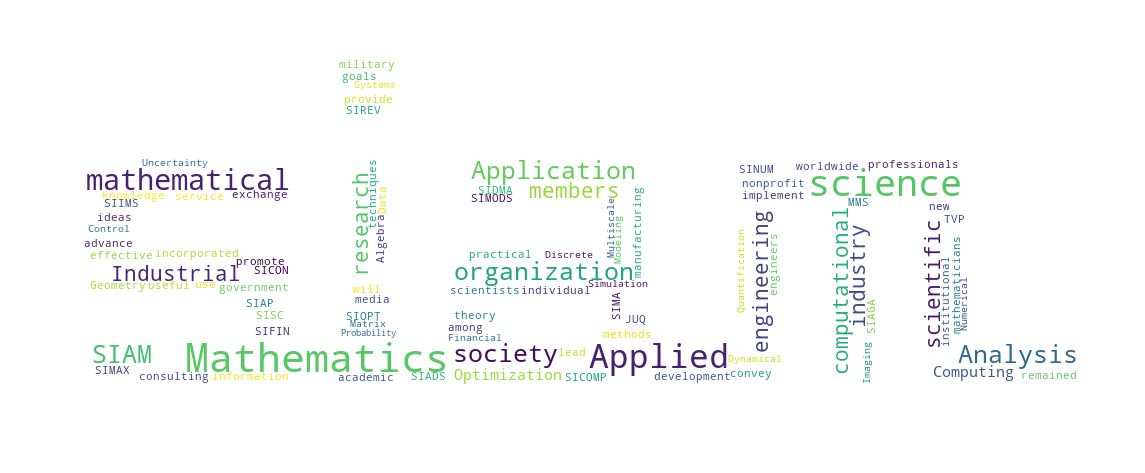
\includegraphics[width=9cm]{a}
  \caption{fig}
\end{figure}
\begin{figure}[H]
  \centering
  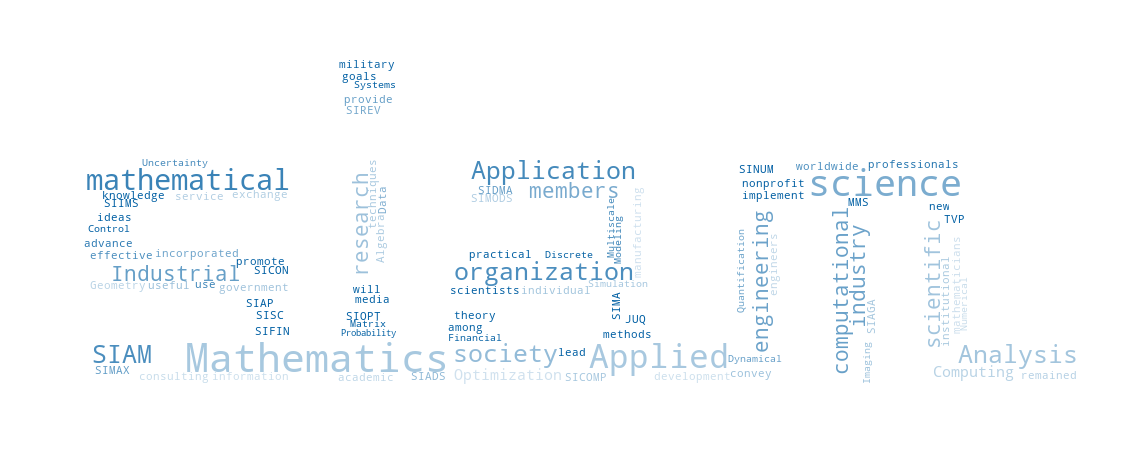
\includegraphics[width=9cm]{b}
  \caption{sfd}
\end{figure}
\begin{table}[H]
  \centering
  \begin{tabular}{rl}
    a&ads
  \end{tabular}
  \caption{as}
\end{table}
\begin{table}[H]
  \centering
  \begin{tabular}{rl}
    a&ads
  \end{tabular}
  \caption{as}
\end{table}

\begin{table}[H]
  \centering
  \begin{tabular}{rl}
    a&ads
  \end{tabular}
  \caption{asasd}
\end{table}
\begin{Algorithm}[H]
    \SetKwFunction{Sum}{sum} % use to define a function name
    \BlankLine
    \Input{Parameters: $i$.}
    \Output{Result: $s$.}
    \BlankLine
    $I\gets \{1,2,3,\ldots,100\}$ \;
    \BlankLine
    \ForEach{$i\in I$}
    {%
        $L_i \gets i$ \;
        $M_i \gets e^i$ \;
    }
    \BlankLine
    \For{$i=1$ \KwTo $100$}
    {%
         $p^i \gets \Sum( l_i,M_i)$ \;
        \If{$i$ is even}
        {%
            $p_i\gets p_i-1$ \;
        }
    }
    \BlankLine
    \For{$i=1: 100$}
    {%
        $q^i \gets \Sum(e^{l_i},e^{M_i})$ \;
        \If{$i$ is even}
        {%
            $q_i\gets p_i-1$ \;
        }
    }
    \While{$i\neq 2$}{$i=i+1$}
     $s\gets p^i+q^i$
    \caption{A example of the algorithms}
    \label{algo:Ch6-ShapeGen}
\end{Algorithm}
\lstinputlisting[language=Matlab,caption={matlab code}]{nearest_product.m}  %% donot need add the parentpath
%%% Local Variables:
%%% mode: latex
%%% TeX-master: "thesis"
%%% End:
\chapter{figures and tables}
\begin{figure}[H]
  \centering
  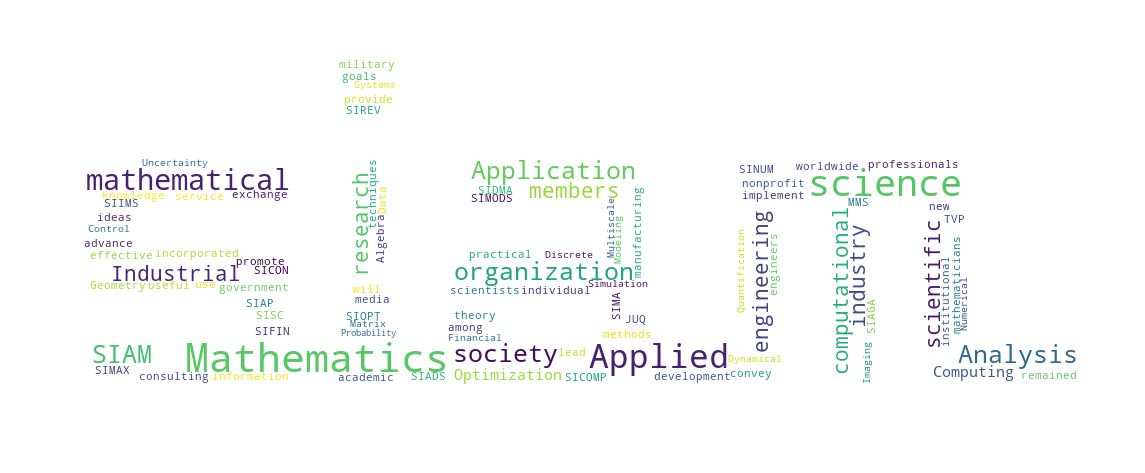
\includegraphics[width=9cm]{a}
  \caption{fig}
\end{figure}
\begin{figure}[H]
  \centering
  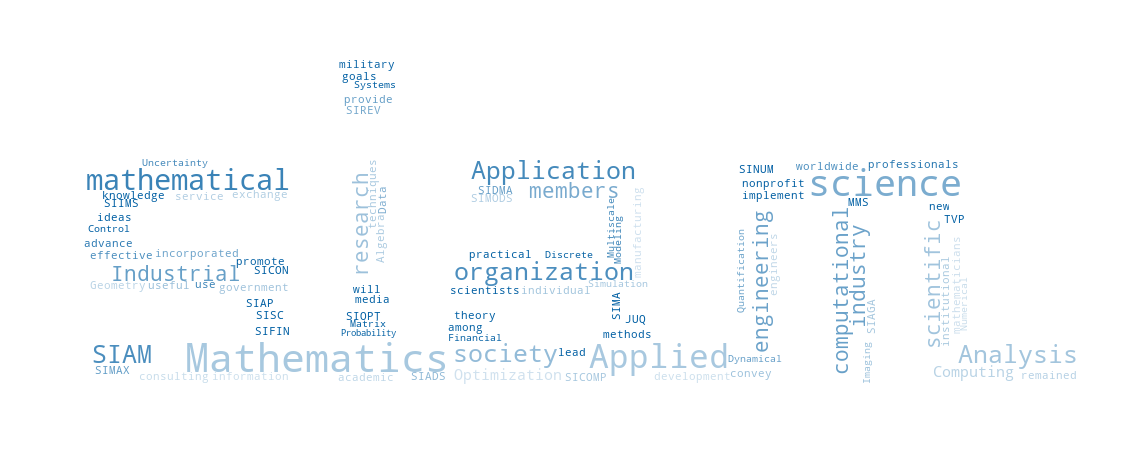
\includegraphics[width=9cm]{b}
  \caption{sfd}
\end{figure}
\begin{table}[H]
  \centering
  \begin{tabular}{rl}
    a&ads
  \end{tabular}
  \caption{as}
\end{table}
\begin{table}[H]
  \centering
  \begin{tabular}{rl}
    a&ads
  \end{tabular}
  \caption{as}
\end{table}

\begin{table}[H]
  \centering
  \begin{tabular}{rl}
    a&ads
  \end{tabular}
  \caption{asasd}
\end{table}
\begin{Algorithm}[H]
    \SetKwFunction{Sum}{sum} % use to define a function name
    \BlankLine
    \Input{Parameters: $i$.}
    \Output{Result: $s$.}
    \BlankLine
    $I\gets \{1,2,3,\ldots,100\}$ \;
    \BlankLine
    \ForEach{$i\in I$}
    {%
        $L_i \gets i$ \;
        $M_i \gets e^i$ \;
    }
    \BlankLine
    \For{$i=1$ \KwTo $100$}
    {%
         $p^i \gets \Sum( l_i,M_i)$ \;
        \If{$i$ is even}
        {%
            $p_i\gets p_i-1$ \;
        }
    }
    \BlankLine
    \For{$i=1: 100$}
    {%
        $q^i \gets \Sum(e^{l_i},e^{M_i})$ \;
        \If{$i$ is even}
        {%
            $q_i\gets p_i-1$ \;
        }
    }
    \While{$i\neq 2$}{$i=i+1$}
     $s\gets p^i+q^i$
    \caption{A example of the algorithms}
    \label{algo:Ch6-ShapeGen}
\end{Algorithm}
\lstinputlisting[language=Matlab,caption={matlab code}]{nearest_product.m}  %% donot need add the parentpath
%%% Local Variables:
%%% mode: latex
%%% TeX-master: "thesis"
%%% End:         % for testing
%% for testing list of symbols
%% To add the symbols to the list of symbols, need to use $\gls{t}$ in the contents
%% which will create hyperlink to the section of listofsymbols
%% To add the description of the symbols, one must add the entry in "symbols.tex" file
\chapter{Sample}
Reference symbols: $\gls{x}$, $\gls{v}$, $\gls{a}$, $\gls{t}$,
$\gls{F}$,$\gls{xx}$.

%%%%%%%%%%%%%%%%%%%%%%%%%%%%%%%%%%%%%%%%%%%%%%%%%%%%%%%%%%%%%%%%%%%%%%%%%%%%%%% 
% bibliography                                                                %
%%%%%%%%%%%%%%%%%%%%%%%%%%%%%%%%%%%%%%%%%%%%%%%%%%%%%%%%%%%%%%%%%%%%%%%%%%%%%%% 
\bibliographystyle{tsien} % bibliography style, for example: plain, style "tsien" is user cumstomized
\bibliography{biblio}       % bib file name 

\end{document}
%%% the following three lines of comments are used for emacs auctex users, each 
%%% input file contains them. One can compile tex file on any buffer of them

%%% Local Variables:
%%% mode: latex
%%% TeX-master: t
%%% End:
